\documentclass[conference]{IEEEtran}
\pagestyle{plain}

\usepackage{graphicx}
\graphicspath{{./imagenes/}{../imagenes/}}
\DeclareGraphicsExtensions{.pdf,.jpeg,.png}
\usepackage[utf8]{inputenc}
\usepackage[T1]{fontenc}
\usepackage{microtype}
\usepackage{xcolor}
\usepackage[cmex10]{amsmath}
\usepackage{amssymb}
\usepackage{siunitx}
\usepackage{float}
\usepackage{array}
\usepackage{url}
\usepackage{makecell}
\usepackage{booktabs}
\usepackage{hyperref}
\usepackage{circuitikz}
\usepackage{tikz}
\usetikzlibrary{shapes.geometric, arrows, arrows.meta, positioning, calc, fit, backgrounds}
\usepackage{etoolbox}
\makeatletter
\apptocmd\@makecaption{\par}{}{}
\makeatother
\usepackage{listings}
\lstset{
    language=Matlab,
    basicstyle=\ttfamily\scriptsize,
    keywordstyle=\color{blue!80!black}\bfseries,
    commentstyle=\color{green!50!black}\itshape,
    stringstyle=\color{purple},
    breaklines=true,
    numbers=left,
    numberstyle=\tiny\color{gray!80},
    numbersep=5pt,
    xleftmargin=18pt,
    xrightmargin=2pt,
    frame=single,
    rulecolor=\color{gray!40},
    backgroundcolor=\color{gray!3},
    captionpos=b,
    inputencoding=utf8,
    extendedchars=true,
    literate={á}{{\'a}}1 {é}{{\'e}}1 {í}{{\'i}}1 {ó}{{\'o}}1 {ú}{{\'u}}1 {ñ}{{\~n}}1 {Á}{{\'A}}1 {É}{{\'E}}1 {Í}{{\'I}}1 {Ó}{{\'O}}1 {Ú}{{\'U}}1 {Ñ}{{\~N}}1
}

\def\figureautorefname{Figura}
\def\equationautorefname{Ecuación}
\def\tableautorefname{Tabla}
\def\sectionautorefname{Sección}
\def\subsectionautorefname{Sección}
\def\subsubsectionautorefname{Sección}
\def\appendixautorefname{Apéndice}
\renewcommand{\lstlistingname}{Código}
\def\lstlistingautorefname{Código}

\IEEEoverridecommandlockouts{}

\tolerance=10000
\hbadness=10000
\emergencystretch=10pt

\begin{document}

\title{Implementación Computacional de Control Directo de Par (DTC), Diagnóstico Predictivo de Fallas con Inteligencia Artificial y Ruta de Mantenimiento para un Motor de Inducción en AgroMolinos del Valle S.A.}

\author{
    \IEEEauthorblockN{H. García, M. Rodríguez y S. Bustamante}
    \IEEEauthorblockA{
        \textit{Universidad de los Llanos} \\
        \textit{Villavicencio, Colombia} \\
        {\small \texttt{hfgarcia@unillanos.edu.co} \quad 161004621}\\
        {\small \texttt{marodriguez.payares@unillanos.edu.co} \quad 161004834}\\
        {\small \texttt{sergio.bustamante@unillanos.edu.co} \quad 161005037}
    }
}

\maketitle

\renewcommand\abstractname{Resumen}
\begin{abstract}
En el procesamiento agroindustrial de granos, las fallas mecánicas y el estrés térmico en motores de inducción ocasionan interrupciones imprevistas con elevados costos de parada. Este artículo presenta el diseño, modelado multifísico y validación de una plataforma integral de control y diagnóstico predictivo para un motor de inducción trifásico jaula de ardilla de 10~HP y 460~V operando en la planta de AgroMolinos del Valle S.A. Partiendo de un esquema de Control Directo de Par (DTC) con regulación de velocidad PI en MATLAB/Simulink (\texttt{InductionMachineDTC.slx}), se articulan un modelo térmico por red Cauer y un estimador de vibraciones conforme a ISO 10816-1. A partir de un corpus balanceado de 1200 registros operacionales sintetizados con la dinámica del sistema, se entrenaron dos modelos supervisados: un Perceptrón Multicapa ($8 \to 16 \to 8 \to 4$) optimizado mediante Adam con regularización $L_2$, y una Máquina de Vectores de Soporte (SVM) con kernel RBF. Ambos clasificadores alcanzaron una exactitud del 100\% sobre 240 muestras de prueba ciega, discriminando operación normal, sobrecalentamiento, desbalance eléctrico y fallas mecánicas en rodamientos. El sistema se integró en un panel de control interactivo en MATLAB App Designer, el cual procesa la telemetría en tiempo real y despacha una ruta de mantenimiento preventivo y predictivo alineada con RETIE (Art.~20) e ISO 10816-1.
\end{abstract}

\renewcommand\IEEEkeywordsname{Palabras clave}
\begin{IEEEkeywords}
Control Directo de Par (DTC), Diagnóstico Predictivo, Inteligencia Artificial, MATLAB App Designer, Motor de Inducción, Redes Neuronales, RETIE, Ruta de Mantenimiento, SVM.
\end{IEEEkeywords}

\section{Introducción}
El procesamiento continuo de granos en la industria molinera impone condiciones de trabajo rigurosas sobre los accionamientos electromecánicos principales \cite{moubray1997}. En las instalaciones de la empresa AgroMolinos del Valle S.A., los molinos de martillos operan mediante un motor trifásico de inducción tipo jaula de ardilla de 10~HP a 460~V, sometido a fluctuaciones estocásticas de par provocadas por variaciones en la densidad y caudal de alimentación de cereal \cite{nandi2005}. Las anomalías incipientes no detectadas, tales como el desbalance entre fases, la pérdida gradual de aislamiento en devanados o el desgaste localizado en pistas de rodamientos, suelen derivar en paradas intempestivas de alto costo y riesgo de atascamiento en tolva \cite{gao2015}.

Para responder a estos requerimientos operativos, los métodos tradicionales de control escalar Voltaje/Frecuencia ($V/f$) presentan limitaciones debido a su lenta respuesta transitoria y su propensión a caídas de velocidad ante impactos repentinos de carga \cite{bose2006}. Por el contrario, la estrategia de Control Directo de Par (DTC) desacopla el flujo magnético estatórico del par electromagnético mediante tablas de conmutación óptima, logrando tiempos de restablecimiento inferiores a $15$~ms sin requerir codificadores mecánicos en el eje \cite{takahashi1986, vas1998}.

En este contexto, este artículo desarrolla la segunda fase del sistema integral de accionamiento, diagnóstico predictivo y mantenimiento para el motor de 10~HP de AgroMolinos del Valle S.A. Las principales contribuciones comprenden: 1) el modelado multifísico acoplado en MATLAB/Simulink integrando el convertidor de potencia, el núcleo DTC, la carga de molienda, la red térmica Cauer y la cinemática de vibraciones; 2) la formulación de un vector de 8 características con normalización $Z$-score y la comparación analítica de clasificadores supervisados (MLP frente a SVM RBF) que alcanzan separación completa de fallas; 3) el diseño de una ruta técnica de mantenimiento preventiva y correctiva basada en RETIE e ISO 10816-1; y 4) el despliegue de una consola gráfica en MATLAB App Designer que sincroniza los parámetros maestros del motor con la inferencia en tiempo real.

\section{Marco Teórico y Fundamentos}

\subsection{Dinámica del Motor de Inducción Trifásico}
El motor de inducción con rotor en jaula de ardilla es el actuador más difundido en accionamientos industriales debido a su robustez estructural, bajo costo y confiabilidad \cite{chapman2012}. La interacción del campo magnético giratorio estatórico, cuya velocidad síncrona ($n_s$) depende de la frecuencia de alimentación y del número de polos (\autoref{eq:ns}), con las corrientes inducidas en las barras rotóricas, produce el par electromagnético necesario para arrastrar la carga mecánica \cite{fitzgerald2003, krishnan2001}:
\begin{equation}
    n_s = \frac{120 f}{P} \quad ; \quad s = \frac{n_s - n_r}{n_s}
    \label{eq:ns}
\end{equation}
El modelado transitorio y la sintonización de lazos de control dinámico requieren proyectar las ecuaciones diferenciales de la máquina sobre un marco de referencia ortogonal ($d-q$) en coordenadas estacionarias o síncronas \cite{leonhard2001}. Asimismo, el circuito equivalente clásico permite desacoplar y calcular los parámetros circuitales fundamentales (resistencias e inductancias de dispersión) que alimentan la simulación computacional \cite{ieee112}.

\subsection{Estrategia de Control Directo de Par (DTC)}
A diferencia de los esquemas orientados por campo (FOC) que dependen de complejas transformaciones de coordenadas y moduladores PWM, el Control Directo de Par (DTC), formulado por Takahashi y Depenbrock \cite{takahashi1986, depenbrock1988}, selecciona de forma directa los estados de conmutación del inversor a partir de los errores instantáneos de par electromagnético y flujo magnético estatórico \cite{vas1998}.

En esta topología, las corrientes y tensiones de fase se miden para reconstruir el vector espacial de flujo estatórico y el par en el plano estacionario $(\alpha, \beta)$ \cite{kazmierkowski2002}. Los errores respecto a sus consignas de referencia alimentan comparadores de histéresis de dos o tres niveles, cuyas salidas digitales, combinadas con la identificación del sector angular, indexan una tabla de conmutación óptima (LUT) que comanda los seis IGBTs del inversor \cite{bose2001}. Esto asegura una respuesta dinámica sumamente ágil ante impactos de molienda, prescindiendo de sensores rotatorios en el eje (operación \textit{sensorless}).

\subsection{Función de Transferencia y Lazo de Velocidad PI}
Aunque el par electromagnético ($T_{em}$) se controla directamente en el bucle interno de histéresis, la velocidad del rotor ($\omega_r$) debe mantenerse regulada frente a las perturbaciones de carga mediante un lazo externo. Para ello se incorpora un compensador Proporcional-Integral (PI) que anula el error de velocidad en régimen permanente y suministra la consigna de par de referencia ($T_{ref}$) al núcleo DTC \cite{ong1998}.

La sintonización analítica de este regulador requiere formular la función de transferencia de la planta mecánica rotacional. A partir de la ecuación de balance de par y considerando una prueba de lazo abierto con par de carga nulo ($T_L = 0$), se obtiene en el dominio de Laplace:
\begin{equation}
    T_{em}(s) = (J s + F) \omega_r(s) \implies G_p(s) = \frac{\omega_r(s)}{T_{em}(s)} = \frac{1}{J s + F}
    \label{eq:tf_planta}
\end{equation}
donde $J$ es la inercia total equivalente y $F$ el coeficiente de fricción viscosa. Al cerrar el lazo con el controlador $C(s) = K_p + K_i/s$, la función de transferencia de lazo cerrado adopta una estructura canónica de segundo orden:
\begin{equation}
    H(s) = \frac{C(s) G_p(s)}{1 + C(s) G_p(s)} = \frac{\frac{K_p s + K_i}{J}}{s^2 + \frac{F + K_p}{J} s + \frac{K_i}{J}}
    \label{eq:tf_lazocerrado}
\end{equation}
Igualando el polinomio característico con la forma estándar $s^2 + 2\zeta\omega_n s + \omega_n^2$, e imponiendo una respuesta críticamente amortiguada ($\zeta = 1.0$) para evitar sobreoscilaciones mecánicas en la transmisión de engranajes, se deducen las ganancias del regulador:
\begin{equation}
    K_p = 2\zeta\omega_n J - F \quad ; \quad K_i = J \omega_n^2
    \label{eq:kp_ki}
\end{equation}
Estas expresiones sustentan el script de sintonización \texttt{tune\_pi.m}, el cual evalúa diferentes anchos de banda ($\omega_n$) para garantizar rapidez en la recuperación de velocidad sin inducir saturación excesiva de corriente en el convertidor \cite{krishnan2001}.

\subsection{Monitoreo Predictivo de Condición Operativa}
El servicio continuo en molienda somete a la máquina a esfuerzos electromecánicos y térmicos que aceleran los mecanismos de degradación \cite{toliyat2012}:
\begin{itemize}
    \item \textbf{Vibración Mecánica:} El análisis de las vibraciones en rodamientos y tapas permite diagnosticar desalineación angular, desbalance de masa y defectos incipientes en pistas de cojinetes. La norma ISO 10816-1 \cite{iso10816} establece las zonas de severidad admisible para motores de esta potencia.
    \item \textbf{Temperatura Estatórica:} El registro térmico continuo mediante sensores RTD tipo PT100 protege el aislamiento de los devanados. Temperaturas por encima de $105^\circ$C advierten condiciones de sobrecarga o ventilación obstruida, mientras que el umbral de $155^\circ$C representa el límite absoluto de destrucción térmica para aislamientos Clase F bajo el reglamento RETIE \cite{retie2013, nandi2005}.
    \item \textbf{Calidad de Energía y Armónicos:} La conmutación de alta frecuencia en el inversor genera armónicos de corriente que incrementan las pérdidas parásitas. El monitoreo de corriente evalúa tanto el desbalance de fases ($IUF$) como la distorsión armónica total ($THD_i$), en concordancia con IEEE 519 \cite{ieee519}.
\end{itemize}

\subsection{Técnicas de Inteligencia Artificial para el Diagnóstico Predictivo de Fallas}
\label{sec:teoria_ia}
Los esquemas convencionales de mantenimiento basados en umbrales estáticos sobre una única variable resultan susceptibles a falsas alarmas ante fluctuaciones operacionales de la molienda \cite{soualhi2022, gao2015}. Por el contrario, los modelos de aprendizaje computacional supervisado procesan vectores multivariables de características, aprendiendo fronteras de decisión no lineales que separan con precisión las condiciones operativas de la máquina.

\subsubsection{Perceptrón Multicapa (MLP) y Regularización}
El Perceptrón Multicapa es una red neuronal prealimentada compuesta por capas densas. La propagación hacia adelante en la capa $l$ transforma las activaciones de la capa anterior $\mathbf{a}^{(l-1)}$ mediante los pesos $\mathbf{W}^{(l)}$, el sesgo $\mathbf{b}^{(l)}$ y una función de activación no lineal $f(z)$:
\begin{equation}
    \mathbf{z}^{(l)} = \mathbf{W}^{(l)} \mathbf{a}^{(l-1)} + \mathbf{b}^{(l)} \quad ; \quad \mathbf{a}^{(l)} = f(\mathbf{z}^{(l)})
    \label{eq:mlp_forward}
\end{equation}
En las capas ocultas se aplica la función ReLU, $f(z) = \max(0, z)$, para mitigar la saturación de gradientes. En la capa de salida ($L$), para un problema con $K$ clases, la función Softmax genera un vector de probabilidades normalizadas $\mathbf{p} \in [0, 1]^K$ ($\sum_{k=1}^K p_k = 1$):
\begin{equation}
    P(y = c \mid \mathbf{x}) = \frac{\exp(z_c^{(L)})}{\sum_{k=1}^K \exp(z_k^{(L)})}
    \label{eq:softmax_teoria}
\end{equation}
El entrenamiento minimiza la función de pérdida de entropía cruzada multiclase con regularización de Tikhonov ($L_2$) para evitar sobreajuste:
\begin{equation}
    \mathcal{L} = -\frac{1}{M}\sum_{i=1}^M \sum_{c=1}^K y_{ic} \ln(p_{ic}) + \frac{\lambda}{2}\sum_{l=1}^L \|\mathbf{W}^{(l)}\|_F^2
    \label{eq:loss_cross_entropy}
\end{equation}

\subsubsection{Máquinas de Vectores de Soporte (SVM) y Kernel RBF}
La Máquina de Vectores de Soporte determina el hiperplano óptimo $\mathbf{w}^T \phi(\mathbf{x}) + b = 0$ que maximiza el margen geométrico entre clases \cite{gangsar2020}. En su formulación dual con parámetro de penalización de holguras $C > 0$:
\begin{equation}
    \max_{\boldsymbol{\alpha}} \sum_{i=1}^M \alpha_i - \frac{1}{2}\sum_{i=1}^M \sum_{j=1}^M \alpha_i \alpha_j y_i y_j K(\mathbf{x}_i, \mathbf{x}_j)
    \label{eq:svm_dual}
\end{equation}
sujeto a $0 \le \alpha_i \le C$ y $\sum_{i=1}^M \alpha_i y_i = 0$. La no linealidad del espacio de fallas se aborda mediante la función de base radial (RBF):
\begin{equation}
    K(\mathbf{x}_i, \mathbf{x}_j) = \exp\left(-\gamma \|\mathbf{x}_i - \mathbf{x}_j\|^2\right)
    \label{eq:rbf_kernel}
\end{equation}
donde $\gamma$ controla el ancho del núcleo gaussiano. La clasificación de cuatro clases se resuelve mediante un esquema One-vs-Rest (OvR).

\subsubsection{Análisis de Componentes Principales (PCA)}
Para evaluar la redundancia y verificar analíticamente la separabilidad del espacio sensorial, se aplica el Análisis de Componentes Principales (PCA). A partir de la matriz centrada $\mathbf{X}_c \in \mathbb{R}^{M \times D}$, la matriz de covarianza $\boldsymbol{\Sigma} = \frac{1}{M-1} \mathbf{X}_c^T \mathbf{X}_c$ se descompone en autovalores y autovectores:
\begin{equation}
    \boldsymbol{\Sigma} \mathbf{v}_k = \lambda_k \mathbf{v}_k \quad (k = 1, \dots, D)
    \label{eq:pca_eigen}
\end{equation}
La proyección sobre los dos primeros componentes ($PC_1, PC_2$) permite comprobar visualmente si los estados de falla forman agrupamientos disjuntos con alta varianza explicada.

\section{Metodología e Infraestructura de Simulación}

La metodología computacional implementada se estructura en tres componentes acoplados en MATLAB/Simulink: el archivo maestro de constantes (\texttt{InductionMachineDTCData.m}), el script de cálculo analítico del lazo PI (\texttt{tune\_pi.m}) y el modelo dinámico multifísico (\texttt{InductionMachineDTC.slx}).

\subsection{Archivo Maestro de Parámetros y Consistencia del Sistema}
Para asegurar la consistencia numérica en todos los módulos (simulador en Simulink, sintetizador de fallas, clasificadores de IA y consola gráfica), el script \texttt{InductionMachineDTCData.m} actúa como fuente centralizada de parámetros (anexado en el \hyperref[app:dtcdata]{Apéndice~\ref*{app:dtcdata}}).

Este archivo define las magnitudes de placa del motor de inducción jaula de ardilla (10~HP, 460~V, 60~Hz, 4 polos), normalizadas bajo el sistema por unidad (p.u.), y calcula analíticamente las magnitudes base de tensión de pico línea-neutro ($V_{base} = V_n \sqrt{2/3} = 375.59$~V), corriente de pico activa ($I_{base} = P_n / (1.5 V_{base}) = 13.24$~A), impedancia base ($Z_{base} = 28.36\,\Omega$) y par electromagnético base ($T_{base} = P_n / (\omega_{base}/p) = 39.58\,\text{N\,m}$). Asimismo, establece el paso de integración rígido ($T_s = 5\,\mu\text{s}$), la frecuencia de conmutación ($f_{sw} = 2$~kHz) y los anchos de histéresis de flujo ($0.015$~Wb) y par ($3.0\,\text{N\,m}$). En la \autoref{tab:parametros} se resumen las constantes eléctricas y mecánicas de la máquina.

\begin{table}[H]
    \centering
    \caption{Parámetros de la Máquina de Inducción de AgroMolinos del Valle S.A.}
    \resizebox{\columnwidth}{!}{
    \begin{tabular}{@{}lcl@{}}
        \toprule
        \textbf{Parámetro} & \textbf{Valor} & \textbf{Significado Físico / Rol en el Modelo} \\ \midrule
        $P_n$ & $7460$ W & Potencia mecánica útil en el eje (10 HP) \\
        $V_n$ & $460$ V & Tensión eficaz nominal de línea (60 Hz) \\
        $f_n$ & $60$ Hz & Frecuencia fundamental del sistema \\
        $R_s$ & $0.0139$ p.u. & Resistencia óhmica estatórica ($0.394\,\Omega$) \\
        $L_{ls}$ & $0.0672$ p.u. & Inductancia de fuga estatórica ($5.05$ mH) \\
        $R_r$ & $0.0112$ p.u. & Resistencia rotórica referida ($0.318\,\Omega$) \\
        $L_{lr}$ & $0.0672$ p.u. & Inductancia de fuga rotórica ($5.05$ mH) \\
        $L_m$ & $2.717$ p.u. & Inductancia mutua de magnetización ($204.4$ mH) \\
        $H$ & $0.2734$ s & Constante de inercia mecánica normalizada \\
        $F$ & $0.0106$ p.u. & Coeficiente de fricción por ventilación y roce \\
        $p$ & $2$ & Pares de polos magnéticos ($n_s = 1800$ RPM) \\ \bottomrule
    \end{tabular}
    }
    \label{tab:parametros}
\end{table}

\subsection{Sintonización Analítica del Regulador de Velocidad PI}
Para fijar el par de referencia del núcleo DTC, el script \texttt{tune\_pi.m} (anexado en el \hyperref[app:tunepi]{Apéndice~\ref*{app:tunepi}}) extrae los parámetros inerciales ($H$) y de amortiguamiento viscoso ($F$) de \texttt{InductionMachineDTCData.m}, los escala a unidades SI ($J = 0.1147\,\text{kg\,m}^2$, $F_{si} = 0.0022\,\text{N\,m\,s/rad}$) y resuelve la asignación de polos en lazo cerrado (\autoref{eq:kp_ki}) para garantizar un amortiguamiento crítico ($\zeta = 1.0$), impidiendo oscilaciones mecánicas perjudiciales en la molienda.

\subsection{Estructura de Control Directo de Par y Modelo Simulink}
La \autoref{fig:control_dtc_tikz} presenta el diagrama de bloques funcional del esquema de control DTC y lazo de velocidad. A partir de las corrientes $i_{abc}$ y tensiones estimadas $v_{abc}$, el estimador calcula el flujo estatórico en coordenadas estacionarias $(\psi_\alpha, \psi_\beta)$, su módulo $|\boldsymbol{\psi}_s|$, el ángulo de fase y el par instantáneo $T_e$. Dos comparadores de histéresis (dos niveles para flujo y tres niveles para par) determinan las banderas digitales $d_\psi$ y $d_T$, las cuales indexan la tabla de conmutación óptima junto al sector espacial $S_k \in \{1, \dots, 6\}$. Los pulsos resultantes comandan el inversor trifásico (VSI) de transistores IGBTs.

\begin{figure}[H]
\centering
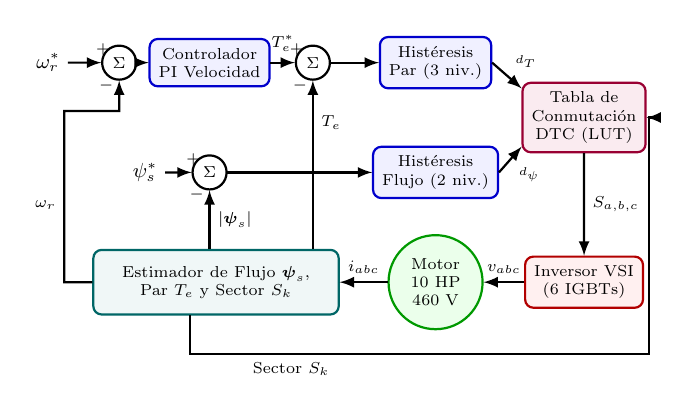
\begin{tikzpicture}[
    >=latex,
    scale=0.82,
    every node/.style={transform shape},
    block/.style={rectangle, draw=blue!80!black, fill=blue!6, thick, rounded corners=3pt, align=center, inner sep=4pt, font=\scriptsize},
    sum/.style={circle, draw=black, thick, fill=white, inner sep=1.2pt, minimum size=15pt, font=\scriptsize},
    tableblock/.style={rectangle, draw=purple!80!black, fill=purple!8, thick, rounded corners=3pt, align=center, inner sep=4pt, font=\scriptsize},
    inverter/.style={rectangle, draw=red!70!black, fill=red!6, thick, rounded corners=3pt, align=center, inner sep=4pt, font=\scriptsize},
    motor/.style={circle, draw=green!60!black, fill=green!8, thick, inner sep=4pt, font=\scriptsize, align=center},
    est/.style={rectangle, draw=teal!80!black, fill=teal!6, thick, rounded corners=3pt, align=center, inner sep=4pt, font=\scriptsize, minimum width=3.8cm, minimum height=1.0cm}
]

% Fila 3: Lazo de Velocidad y Par (Y = 4.4)
\node (wref) at (0.0, 4.4) [font=\small] {$\omega_r^*$};
\node[sum] (sum_w) at (1.1, 4.4) {$\Sigma$};
\node at (0.85, 4.6) [font=\scriptsize\bfseries] {$+$};
\node at (0.9, 4.05) [font=\scriptsize\bfseries] {$-$};

\node[block] (pi) at (2.5, 4.4) {Controlador\\PI Velocidad};

\node[sum] (sum_t) at (4.1, 4.4) {$\Sigma$};
\node at (3.85, 4.6) [font=\scriptsize\bfseries] {$+$};
\node at (3.9, 4.05) [font=\scriptsize\bfseries] {$-$};

\node[block] (hyst_t) at (6.0, 4.4) {Hist\'eresis\\Par ($3$ niv.)};

% Fila 2: Lazo de Flujo Estatórico (Y = 2.7)
\node (psiref) at (1.5, 2.7) [font=\small] {$\psi_s^*$};
\node[sum] (sum_p) at (2.5, 2.7) {$\Sigma$};
\node at (2.25, 2.9) [font=\scriptsize\bfseries] {$+$};
\node at (2.3, 2.35) [font=\scriptsize\bfseries] {$-$};

\node[block] (hyst_p) at (6.0, 2.7) {Hist\'eresis\\Flujo ($2$ niv.)};

% Tabla de Conmutación DTC (Y = 3.55)
\node[tableblock] (lut) at (8.3, 3.55) {Tabla de\\Conmutaci\'on\\DTC (LUT)};

% Fila 1: Etapa de Potencia, Motor y Estimador (Y = 1.0)
\node[inverter] (inv) at (8.3, 1.0) {Inversor VSI\\(6 IGBTs)};
\node[motor] (mot) at (6.0, 1.0) {Motor\\10 HP\\460 V};
\node[est] (estim) at (2.6, 1.0) {Estimador de Flujo $\boldsymbol{\psi}_s$,\\Par $T_e$ y Sector $S_k$};

% Trayectoria directa de Velocidad y Par
\draw[->, thick] (wref) -- (sum_w.west);
\draw[->, thick] (sum_w.east) -- (pi.west);
\draw[->, thick] (pi.east) -- node[above=1pt, font=\scriptsize] {$T_e^*$} (sum_t.west);
\draw[->, thick] (sum_t.east) -- (hyst_t.west);
\draw[->, thick] (hyst_t.east) -- node[above right, font=\tiny] {$d_T$} (lut.155);

% Trayectoria directa de Flujo
\draw[->, thick] (psiref) -- (sum_p.west);
\draw[->, thick] (sum_p.east) -- (hyst_p.west);
\draw[->, thick] (hyst_p.east) -- node[below right, font=\tiny] {$d_\psi$} (lut.205);

% Conexiones de potencia y sensado
\draw[->, thick] (lut) -- node[right, font=\scriptsize] {$S_{a,b,c}$} (inv);
\draw[->, thick] (inv.west) -- node[above, font=\scriptsize] {$v_{abc}$} (mot.east);
\draw[->, thick] (mot.west) -- node[above, font=\scriptsize] {$i_{abc}$} (estim.east);

% Realimentación 1: Velocidad wr -> sum_w.south (sale a la izquierda a X=0.25 y sube limpia)
\draw[->, thick] (estim.west) -- (0.25, 1.0) -- (0.25, 3.65) node[pos=0.45, left, font=\scriptsize] {$\omega_r$} -| (sum_w.south);

% Realimentación 2: Flujo |psi_s| -> sum_p.south (sube vertical directa en X=2.5 desde estim)
\draw[->, thick] (estim.north -| sum_p.south) -- node[pos=0.5, right, font=\scriptsize] {$|\boldsymbol{\psi}_s|$} (sum_p.south);

% Realimentación 3: Par Te -> sum_t.south (sale directamente del borde superior del bloque estimador en X=4.1)
\draw[->, thick] (estim.north -| sum_t.south) -- node[pos=0.75, right, font=\scriptsize] {$T_e$} (sum_t.south);

% Realimentación 4: Sector Sk -> lut.east (desciende más a la izquierda y etiqueta desplazada hacia la izquierda)
\draw[->, thick] ([xshift=-0.4cm]estim.south) -- ++(0, -0.6) -- node[below, font=\scriptsize, pos=0.22] {Sector $S_k$} ++(7.1, 0) |- (lut.east);

\end{tikzpicture}
\caption{Diagrama de bloques de la estrategia de Control Directo de Par (DTC) y regulaci\'on de velocidad PI.}
\label{fig:control_dtc_tikz}
\end{figure}

En concordancia con este esquema, la \autoref{fig:control_simulink} presenta la implementaci\'on del lazo de control PI de velocidad y generaci\'on de pulsos DTC tal como qued\'o estructurado en el modelo de simulaci\'on en Simulink (\texttt{InductionMachineDTC.slx}). En esta implementaci\'on concreta de la simulaci\'on, la consigna de velocidad atraviesa un limitador de pendiente (\textit{rate limiter} fijado en $2000\,\text{rpm/s}$) y un bloque de saturaci\'on, ingresando en unidades por unidad (p.u.) al punto de suma junto a la velocidad angular retroalimentada $\omega_r$ muestreada por un retenedor de orden cero (\textit{Zero-Order Hold}). El bloque discreto del compensador PI (\texttt{PI (wr)}) genera la se\~nal de par de consigna con protecci\'on anti-windup, la cual se escala mediante $T_{base}$ para ingresar como referencia de par ($T_e^*$) al n\'ucleo de conmutaci\'on DTC y accionar las compuertas del inversor.

\begin{figure}[H]
    \centering
    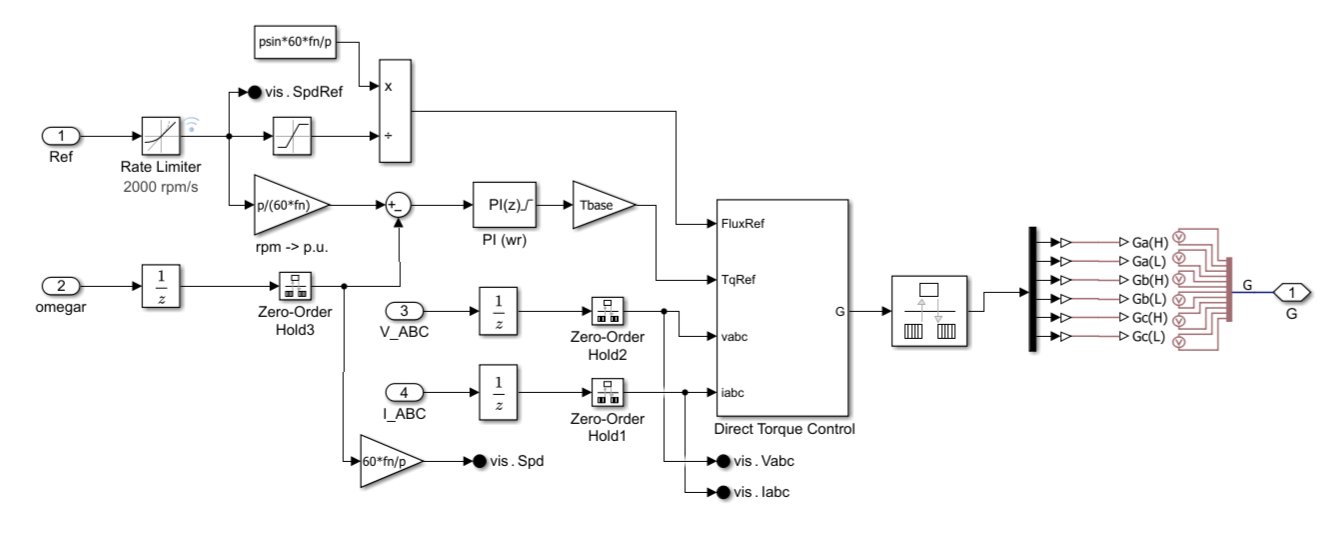
\includegraphics[width=\columnwidth]{control.png}
    \caption{Implementaci\'on del lazo de control PI de velocidad y m\'odulo DTC tal como qued\'o en la simulaci\'on de Simulink.}
    \label{fig:control_simulink}
\end{figure}

La \autoref{fig:circuito} sintetiza la arquitectura multif\'isica y multidominio implementada en Simulink (\texttt{InductionMachineDTC.slx}), articulando sus cinco subsistemas fundamentales: potencia el\'ectrica (red AC de $460$\,V, rectificador, bus DC de $650$\,V e inversor trif\'asico VSI), control DTC y lazo de velocidad PI, acoplamiento electromec\'anico del rotor con la carga din\'amica de molienda, disipaci\'on t\'ermica de p\'erdidas en cobre ($P_{cu} = 3I_s^2 R_s$) v\'ia red Cauer RC equivalente (monitoreo RETIE Clase F), y estimaci\'on de vibraciones estructurales (\autoref{fig:vibraciones_bloque}) bajo la norma ISO 10816-1.

\begin{figure*}[!t]
    \centering
    \resizebox{0.92\textwidth}{!}{%
    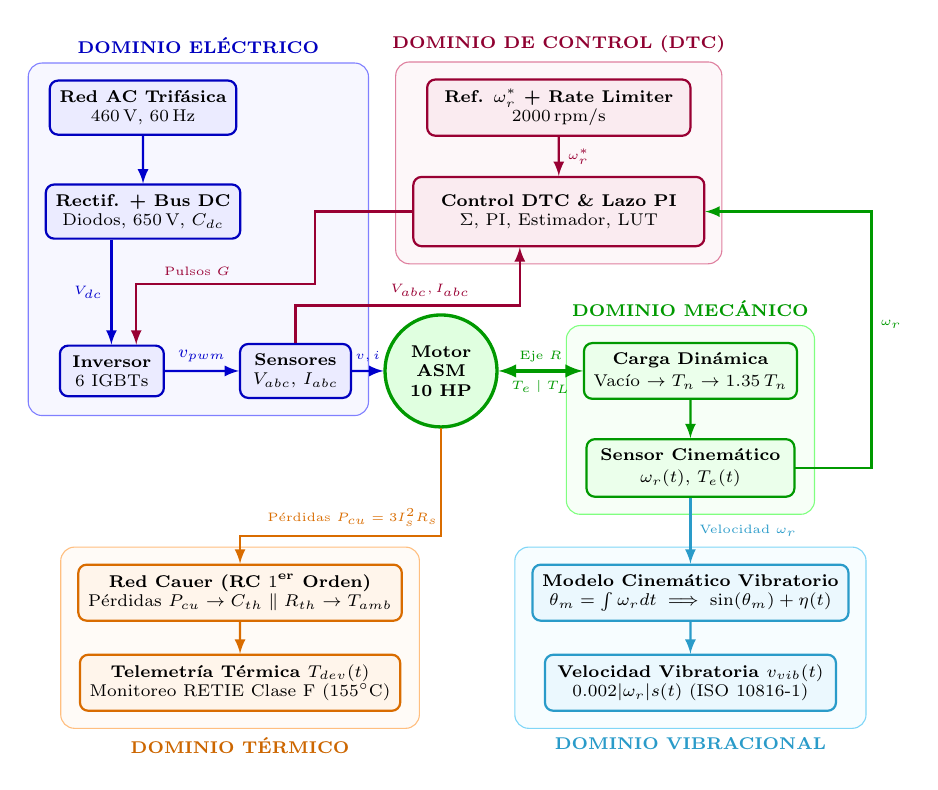
\begin{tikzpicture}[
        >=latex,
        scale=0.88,
        every node/.style={transform shape},
        % Estilos de bloques temáticos
        pwr/.style={rectangle, draw=blue!75!black, fill=blue!8, thick, rounded corners=3pt, align=center, inner sep=4pt, font=\scriptsize},
        ctrl/.style={rectangle, draw=purple!80!black, fill=purple!8, thick, rounded corners=3pt, align=center, inner sep=4pt, font=\scriptsize},
        mot/.style={circle, draw=green!60!black, fill=green!12, very thick, inner sep=2pt, font=\scriptsize\bfseries, align=center, minimum size=46pt},
        mech/.style={rectangle, draw=green!60!black, fill=green!8, thick, rounded corners=3pt, align=center, inner sep=4pt, font=\scriptsize},
        therm/.style={rectangle, draw=orange!85!black, fill=orange!8, thick, rounded corners=3pt, align=center, inner sep=4pt, font=\scriptsize},
        vib/.style={rectangle, draw=cyan!80!black, fill=cyan!8, thick, rounded corners=3pt, align=center, inner sep=4pt, font=\scriptsize}
    ]

    % =========================================================================
    % 1. DOMINIO ELÉCTRICO DE POTENCIA (Columna Izquierda X = 0.6)
    % =========================================================================
    \node[pwr, minimum width=2.4cm] (grid)    at (0.6, 8.8) {\textbf{Red AC Trif\'asica}\\$460$\,V, $60$\,Hz};
    \node[pwr, minimum width=2.4cm] (rectbus) at (0.6, 7.3) {\textbf{Rectif. + Bus DC}\\Diodos, $650$\,V, $C_{dc}$};
    \node[pwr, minimum width=1.5cm] (inv)     at (0.15, 5.0) {\textbf{Inversor}\\$6$ IGBTs};
    \node[pwr, minimum width=1.6cm] (sens)    at (2.8, 5.0) {\textbf{Sensores}\\$V_{abc},\, I_{abc}$};

    % =========================================================================
    % 2. DOMINIO DE CONTROL DTC (Superior Centro X = 6.6)
    % =========================================================================
    \node[ctrl, minimum width=3.8cm] (ref) at (6.6, 8.8) {\textbf{Ref. $\omega_r^*$ + Rate Limiter}\\$2000$\,rpm/s};
    \node[ctrl, minimum width=4.2cm, minimum height=1.0cm] (dtc) at (6.6, 7.3) {\textbf{Control DTC \& Lazo PI}\\$\Sigma$, PI, Estimador, LUT};

    % =========================================================================
    % 3. NÚCLEO MULTIFÍSICO: MOTOR DE INDUCCIÓN (ASM) (Centro X = 4.9)
    % =========================================================================
    \node[mot] (motor) at (4.9, 5.0) {Motor\\ASM\\10 HP};

    % =========================================================================
    % 4. DOMINIO MECÁNICO (Derecha X = 8.5)
    % =========================================================================
    \node[mech, minimum width=3.0cm] (tload) at (8.5, 5.0) {\textbf{Carga Din\'amica}\\[1pt]Vac\'io $\to T_n \to 1.35\,T_n$};
    \node[mech, minimum width=3.0cm] (meas)  at (8.5, 3.6) {\textbf{Sensor Cinem\'atico}\\[1pt]$\omega_r(t),\, T_e(t)$};

    % =========================================================================
    % 5. DOMINIO TÉRMICO (Inferior Izquierda X = 2.0)
    % =========================================================================
    \node[therm, minimum width=4.0cm] (cauer) at (2.0, 1.8) {\textbf{Red Cauer (RC $1^\text{er}$ Orden)}\\P\'erdidas $P_{cu} \to C_{th} \parallel R_{th} \to T_{amb}$};
    \node[therm, minimum width=4.0cm] (temp)  at (2.0, 0.5) {\textbf{Telemetr\'ia T\'ermica $T_{dev}(t)$}\\Monitoreo RETIE Clase F ($155^\circ$C)};

    % =========================================================================
    % 6. DOMINIO DE VIBRACIONES (Inferior Derecha X = 8.5)
    % =========================================================================
    \node[vib, minimum width=4.2cm] (vkin)  at (8.5, 1.8) {\textbf{Modelo Cinem\'atico Vibratorio}\\$\theta_m = \int \omega_r dt \implies \sin(\theta_m) + \eta(t)$};
    \node[vib, minimum width=4.2cm] (vtele) at (8.5, 0.5) {\textbf{Velocidad Vibratoria $v_{vib}(t)$}\\$0.002 |\omega_r| s(t)$ (ISO 10816-1)};

    % =========================================================================
    % CONEXIONES INTERNAS Y MULTIFÍSICAS (ZERO-CROSSING PLANAR)
    % =========================================================================
    % Cadena de potencia eléctrica principal
    \draw[->, thick, blue!80!black] (grid) -- (rectbus);
    \draw[->, thick, blue!80!black] ([xshift=-13pt]rectbus.south) -- node[left, font=\tiny] {$V_{dc}$} ([xshift=-13pt]rectbus.south |- inv.north);
    \draw[->, thick, blue!80!black] (inv) -- node[above, font=\scriptsize] {$v_{pwm}$} (sens);
    \draw[->, thick, blue!80!black] (sens) -- node[above, font=\tiny] {$v, i$} (motor.west);

    % Control DTC: Referencia
    \draw[->, thick, purple!80!black] (ref) -- node[right, font=\tiny] {$\omega_r^*$} (dtc);

    % Disparo de IGBTs (Pulsos G) - Bajado a Y=6.25 (mitad de altura de elevación)
    \draw[->, thick, purple!80!black] (dtc.west) -- ++(-1.4, 0) -- ++(0, -1.05) -| node[pos=0.33, above, font=\tiny] {Pulsos $G$} ([xshift=10pt]inv.north);

    % Medidas V, I hacia Control - Bajado a Y=5.94 (mitad de elevación sobre sensores)
    \draw[->, thick, purple!80!black] (sens.north) -- ++(0, 0.54) -| node[pos=0.30, above, font=\tiny] {$V_{abc}, I_{abc}$} ([xshift=-16pt]dtc.south);

    % Acoplamiento mecánico y feedback cinemático
    \draw[<->, very thick, green!60!black] (motor.east) -- node[above, font=\tiny] {Eje $R$} node[below, font=\tiny] {$T_e \mid T_L$} (tload.west);
    \draw[->, thick, green!60!black] (tload) -- (meas);
    \draw[->, thick, green!60!black] (meas.east) -- ++(1.1, 0) |- node[pos=0.28, right, font=\tiny] {$\omega_r$} (dtc.east);

    % Térmico (Pérdidas Joule en estator)
    \draw[->, thick, orange!85!black] (motor.south) -- ++(0, -1.55) -| node[pos=0.22, above, font=\tiny] {P\'erdidas $P_{cu} = 3I_s^2 R_s$} (cauer.north);
    \draw[->, thick, orange!85!black] (cauer) -- (temp);

    % Vibraciones (Velocidad cinemática de eje directo vertical con amplio despeje)
    \draw[->, thick, cyan!80!black] (meas.south) -- node[right, font=\tiny] {Velocidad $\omega_r$} (vkin.north);
    \draw[->, thick, cyan!80!black] (vkin) -- (vtele);

    % =========================================================================
    % CAJAS DELIMITADORAS DE DOMINIOS (Background)
    % =========================================================================
    \begin{scope}[on background layer]
        % Dominio Eléctrico
        \node[draw=blue!50, fill=blue!3, rounded corners=5pt, fit=(grid)(rectbus)(inv)(sens), inner sep=6pt] (box_elec) {};
        \node[anchor=south, font=\scriptsize\bfseries, text=blue!75!black] at (box_elec.north) {DOMINIO EL\'ECTRICO};
        
        % Dominio Control
        \node[draw=purple!50, fill=purple!3, rounded corners=5pt, fit=(ref)(dtc), inner sep=6pt] (box_ctrl) {};
        \node[anchor=south, font=\scriptsize\bfseries, text=purple!75!black] at (box_ctrl.north) {DOMINIO DE CONTROL (DTC)};
        
        % Dominio Mecánico
        \node[draw=green!50, fill=green!3, rounded corners=5pt, fit=(tload)(meas), inner sep=6pt] (box_mech) {};
        \node[anchor=south, font=\scriptsize\bfseries, text=green!60!black] at (box_mech.north) {DOMINIO MEC\'ANICO};
        
        % Dominio Térmico
        \node[draw=orange!50, fill=orange!3, rounded corners=5pt, fit=(cauer)(temp), inner sep=6pt] (box_therm) {};
        \node[anchor=north, font=\scriptsize\bfseries, text=orange!80!black] at (box_therm.south) {DOMINIO T\'ERMICO};
        
        % Dominio Vibraciones
        \node[draw=cyan!50, fill=cyan!3, rounded corners=5pt, fit=(vkin)(vtele), inner sep=6pt] (box_vib) {};
        \node[anchor=north, font=\scriptsize\bfseries, text=cyan!80!black] at (box_vib.south) {DOMINIO VIBRACIONAL};
    \end{scope}

    \end{tikzpicture}%
    }
    \caption{Arquitectura multif\'isica del modelo de simulaci\'on en Simulink (\texttt{InductionMachineDTC.slx}), integrando los dominios el\'ectrico de potencia, control DTC/PI, acoplamiento mec\'anico, t\'ermico (red Cauer) y vibracional (ISO 10816-1).}
    \label{fig:circuito}
\end{figure*}

\subsection{Metodología de Generación de Datos de Falla, Ingeniería de Características y Preprocesamiento}
\label{sec:metodologia_datos}
La articulación entre el modelo físico en Simulink y la capa de diagnóstico predictivo inteligente requiere un corpus representativo de datos operacionales que capture tanto la variabilidad estocástica del proceso de molienda como las firmas distintivas de degradación electromecánica.

\subsubsection{Generación Fenomenológica del Dataset de Fallas}
Para asegurar coherencia absoluta con los parámetros del motor, el script \texttt{generate\_dataset.m} (anexado en el \hyperref[app:gen]{Apéndice~\ref*{app:gen}}) importa directamente las magnitudes nominales y límites térmicos de \texttt{InductionMachineDTCData.m}. Se sintetizan 1200 registros de operación balanceados (300 muestras por cada estado) que emulan cuatro condiciones críticas de operación:
\begin{enumerate}
    \item \textbf{Clase 1 - Operación Normal (CONFORME):} Funcionamiento con variaciones aleatorias de par de carga en molienda ($20\%$ a $100\%$ de $T_n$), temperatura estabilizada ($45 - 75^\circ$C), corriente balanceada ($IUF < 3\%$, $THD_i < 5\%$) y vibraciones en Zona A/B de ISO 10816-1 ($v_{rms} \le 1.8$ mm/s).
    \item \textbf{Clase 2 - Sobrecalentamiento / Sobrecarga Térmica:} Condición de atascamiento o ventilación forzada defectuosa, con corrientes sostenidas de sobrecarga ($1.1 - 1.4 \times I_n$), temperatura de devanado elevada ($105 - 150^\circ$C, aproximándose al límite RETIE Clase F de $155^\circ$C) y gradiente térmico acelerado ($dT/dt > 1.5^\circ$C/min).
    \item \textbf{Clase 3 - Falla Eléctrica (Asimetría / Espiras en Corto):} Asimetría en los devanados del estator inducida por pérdida parcial de aislamiento entre espiras o desbalance de fases, evidenciada por un factor de desbalance de corriente severo ($IUF = 8\% - 25\%$), presencia de armónicos anómalos ($THD_i = 10\% - 22\%$) y caídas asimétricas de tensión.
    \item \textbf{Clase 4 - Falla Mecánica (Rodamientos / Desalineación):} Degradación acelerada en pistas de rodamientos y desalineación entre el eje motor y los rodillos del molino, generando velocidades eficaces de vibración $v_{rms} = 4.5 - 9.0$ mm/s (Zona C/D de ISO 10816-1) con impactos pico de choque $v_{peak} > 7.0$ mm/s.
\end{enumerate}

\subsubsection{Vector de Características Multidimensional}
A partir del instrumental sensorial disponible en planta y emulado en la simulación, se estructura un vector de características $\mathbf{x} = [x_1, \dots, x_8]^T \in \mathbb{R}^8$:
\begin{enumerate}
    \item $I_{rms}$ [A]: Valor cuadrático medio de la corriente de estator.
    \item $IUF$ [\%]: Factor de desbalance de corriente estatórica, $IUF = \frac{\max(|I_{abc} - I_{avg}|)}{I_{avg}} \times 100$.
    \item $THD_i$ [\%]: Distorsión armónica total de corriente \cite{ieee519}.
    \item $V_{rms}$ [V]: Tensión RMS eficaz línea a línea en bornes.
    \item $T_{dev}$ [$^\circ$C]: Temperatura continua de devanados (red Cauer).
    \item $dT/dt$ [$^\circ$C/min]: Gradiente térmico instantáneo.
    \item $v_{rms}$ [mm/s]: Velocidad eficaz de vibración mecánica en el domo según ISO 10816-1 \cite{iso10816}.
    \item $v_{peak}$ [mm/s]: Amplitud pico de impacto mecánico.
\end{enumerate}

\subsubsection{\texorpdfstring{Estandarización $Z$-Score y Partición Estratificada}{Estandarización Z-Score y Partición Estratificada}}
Dado que las variables presentan rangos de escala dispares (e.g., $V_{rms} \approx 460$ V frente a $v_{rms} \approx 1.2$ mm/s), se aplica una transformación $Z$-Score estricta previa al entrenamiento y la inferencia:
\begin{equation}
    \hat{x}_j = \frac{x_j - \mu_j}{\sigma_j} \quad \forall j \in \{1, \dots, 8\}
    \label{eq:zscore_metodo}
\end{equation}
Para evitar cualquier fuga de información (\textit{data leakage}), la media $\mu_j$ y la desviación estándar $\sigma_j$ se calculan exclusivamente sobre el conjunto de entrenamiento y se almacenan como constantes maestras para el preprocesamiento del conjunto de prueba y la inferencia en tiempo real en la GUI.

El corpus total de 1200 registros se somete a una partición estratificada aleatoria fijando la semilla determinística (\texttt{rng(42)}): el $80\%$ (960 muestras, 240 por clase) se asigna al conjunto de entrenamiento, mientras que el $20\%$ restante (240 muestras, 60 por clase) se reserva estrictamente como conjunto de prueba ciega (\textit{test set}) para la evaluación imparcial de los modelos.

\section{Resultados y Análisis Dinámico}

La validación del modelo se ejecutó directamente sobre el archivo de simulación \texttt{InductionMachineDTC.slx} en el entorno MATLAB/Simulink. La prueba contempla una consigna escalonada de velocidad de $1600$~RPM inyectada en $t = 0.1$~s y la posterior aplicación de un perfil de carga dinámica multifásico (\autoref{fig:carga}), simulando el ciclo operacional del molino de martillos de AgroMolinos del Valle S.A.

\begin{figure}[H]
    \centering
    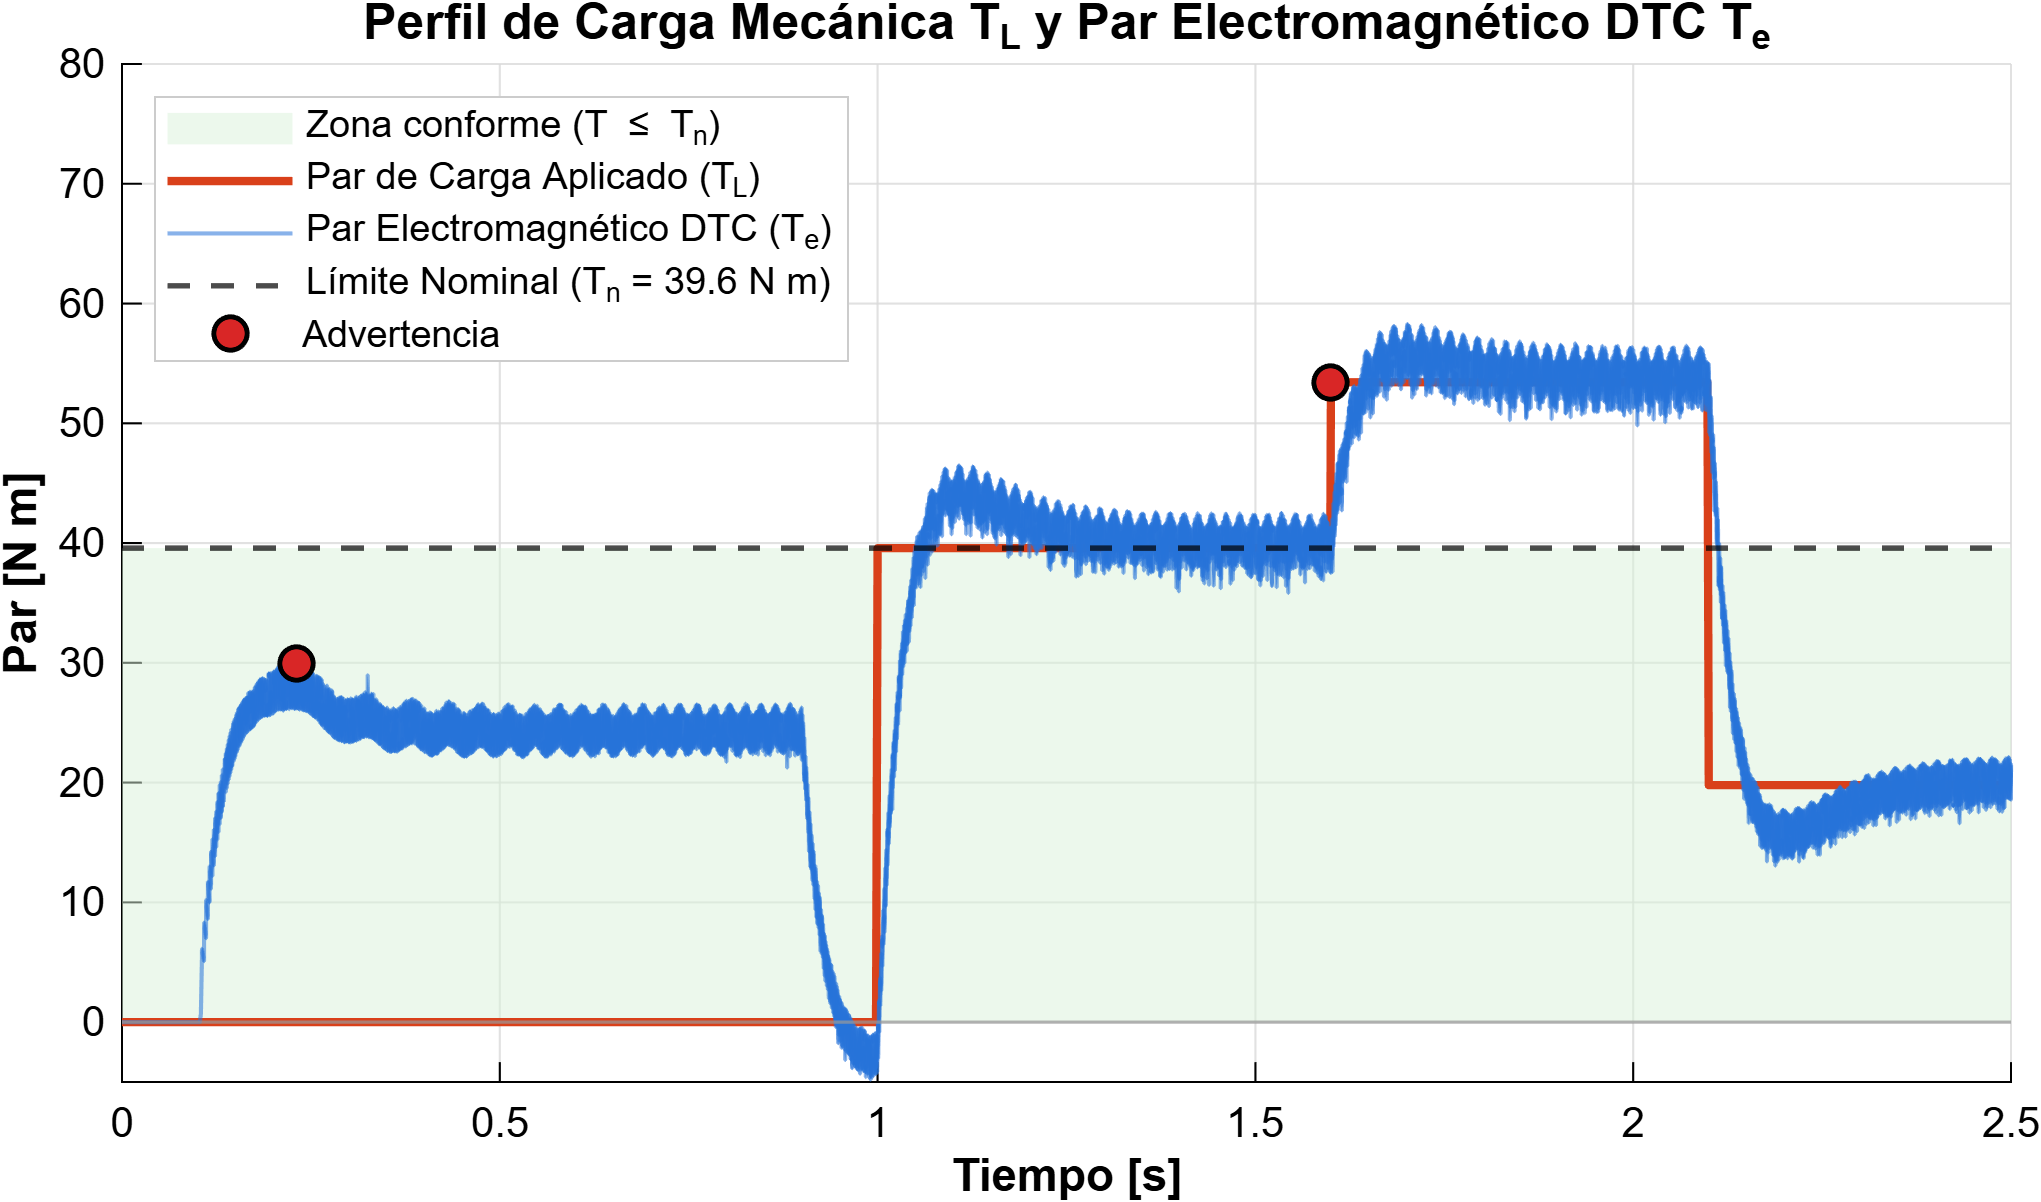
\includegraphics[width=0.92\columnwidth]{carga.png}
    \caption{Perfil de carga mecánica ($T_L$) y par electromagnético DTC ($T_e$) extraído de la simulación de Simulink, delimitando la zona de trabajo conforme ($T \le T_n$, sombreada en verde) y señalando los puntos de advertencia en arranque y sobrecarga por atasco de tolva a $1.35 T_n$.}
    \label{fig:carga}
\end{figure}

Tal como se documenta en la \autoref{fig:carga}, la simulación articula cuatro fases de operación:
\begin{enumerate}
    \item \textbf{Arranque en vacío ($0 \le t < 1.0$~s):} El motor acelera sin carga ($T_L = 0$). El lazo DTC satura su par en el límite dinámico de aceleración ($\approx 28~\text{N\,m}$, indicado con el punto de advertencia), alcanzando los $1600$~RPM en $t \approx 0.85$~s, momento en el cual el par desciende al nivel de fricción en vacío.
    \item \textbf{Molienda nominal en zona conforme ($1.0 \le t < 1.6$~s):} Se aplica el par de molienda nominal ($T_L = T_n = 39.58~\text{N\,m}$). La máquina opera de manera perfectamente estable dentro de la zona de trabajo conforme sombreada en verde, sin registrar alertas.
    \item \textbf{Atasco severo por sobrecarga ($1.6 \le t < 2.1$~s):} Se introduce un ingreso excesivo de grano en la tolva que demanda $T_L = 1.35 T_n = 53.43~\text{N\,m}$. Esta condición excede la capacidad continua nominal, abandonando la zona conforme y activando el punto de advertencia discreto en $t = 1.60$~s.
    \item \textbf{Alivio de carga y recuperación ($2.1 \le t \le 2.5$~s):} Se modela la apertura de compuertas de alivio, reduciendo la carga al $50\%$ ($T_L = 0.5 T_n = 19.79~\text{N\,m}$), retornando de inmediato a la zona segura.
\end{enumerate}

\subsection{Comportamiento Eléctrico y Dinámica de Control}
La respuesta eléctrica ante estos eventos dinámicos se examina en las tensiones y corrientes del estator. La \autoref{fig:voltaje} exhibe el tren de pulsos modulados discretos generados por el inversor trifásico alimentado desde el bus de corriente continua ($V_{dc} = 650$~V). Se presenta un acercamiento en la ventana crítica del escalón de sobrecarga ($t \in [1.58, 1.66]$~s).

\begin{figure}[H]
    \centering
    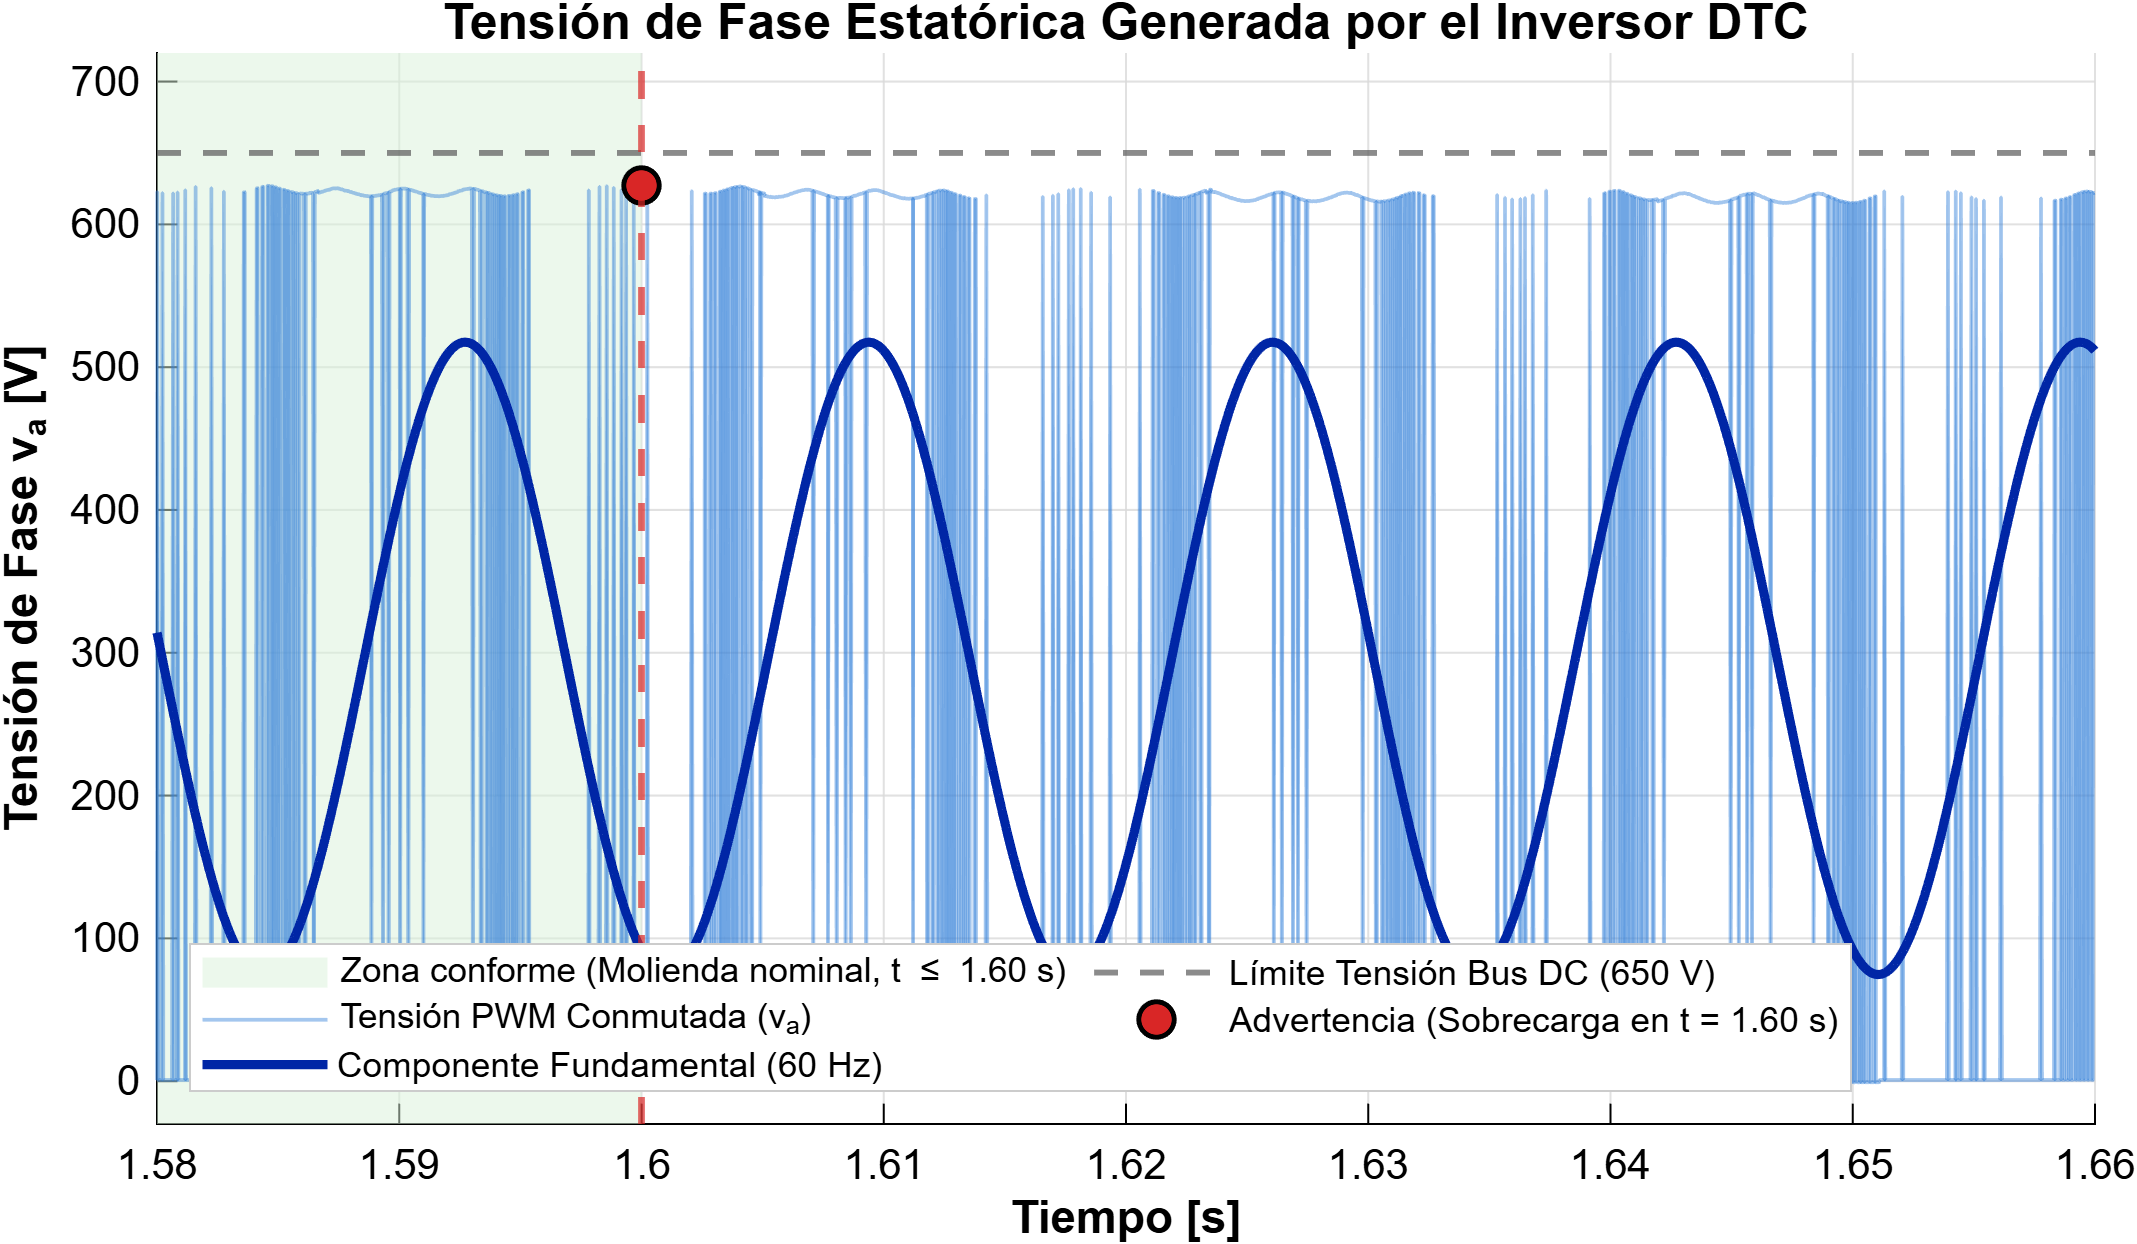
\includegraphics[width=0.92\columnwidth]{voltaje.png}
    \caption{Tensión PWM de fase ($v_a$) y componente fundamental ($60$~Hz) generadas por el inversor DTC en Simulink durante el escalón de sobrecarga ($t \in [1.58, 1.66]$~s), delimitando la zona temporal conforme ($t \le 1.60$~s), el límite físico del bus DC ($650$~V) y el punto de advertencia en $t = 1.60$~s.}
    \label{fig:voltaje}
\end{figure}

En la \autoref{fig:voltaje} se aprecia la delimitación de la zona de operación conforme (molienda nominal para $t \le 1.60$~s), el límite físico superior impuesto por el bus de corriente continua ($V_{dc} = 650$~V) y el punto de advertencia en $t = 1.60$~s marcado sobre la cresta del pulso activo. En este instante, el atasco repentino en la tolva ($1.35 T_n$) genera un error de par que satura el lazo DTC, forzando la supresión de vectores nulos y la aplicación continua de vectores activos para sostener el flujo estatórico. La superposición de la componente fundamental de $60$~Hz evidencia la síntesis armónica lograda por el inversor trifásico.

Las corrientes trifásicas del estator (\autoref{fig:corrientes}) reflejan la delimitación del régimen continuo conforme ($|i| \le I_{peak,nom} \approx 18.7$~A). Se identifican dos puntos de advertencia discretos: en el encendido ($t \approx 0.12$~s), donde la magnetización inicial produce una corriente de inrush transitoria de $I_{peak} \approx 85$~A, y en $t = 1.62$~s, donde el atasco de tolva incrementa la demanda de corriente a $I_{peak} \approx 21.5$~A, superando el límite continuo admisible. Durante el régimen de carga nominal ($1.0 \le t < 1.6$~s), las tres fases permanecen estrictamente confinadas en la franja verde conforme ($I_{peak} \approx 17.5$~A), demostrando equilibrio simétrico y ausencia de perturbaciones.

\begin{figure}[H]
    \centering
    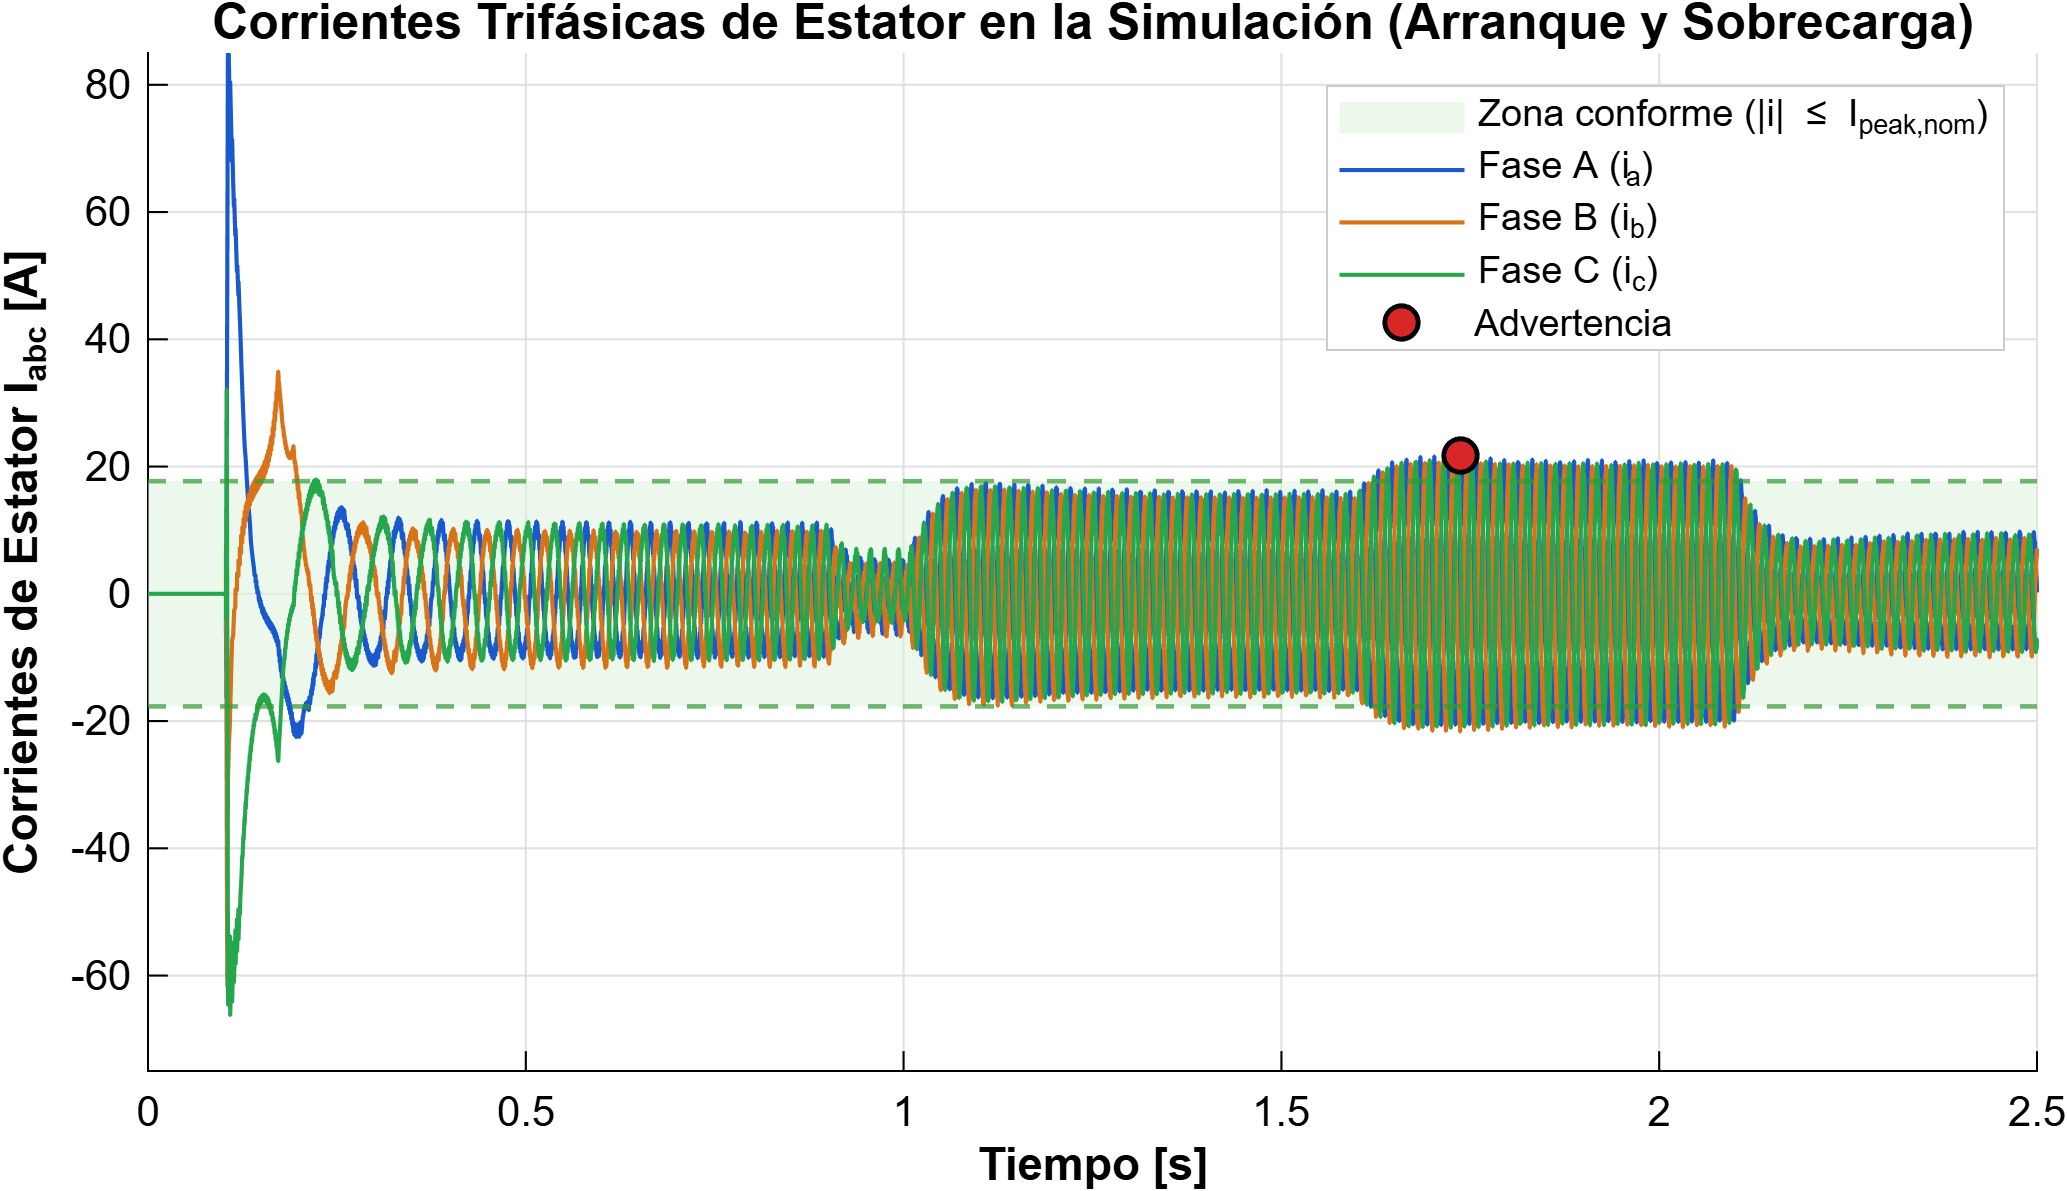
\includegraphics[width=0.92\columnwidth]{corrientes.png}
    \caption{Corrientes trifásicas de estator ($I_{abc}$) obtenidas en Simulink, delimitando la zona conforme de régimen continuo ($|i| \le I_{peak,nom} \approx 18.7$~A) y señalando los puntos de advertencia en arranque y sobrecarga.}
    \label{fig:corrientes}
\end{figure}

En cuanto a la cinemática del rotor, la \autoref{fig:velocidad} demuestra el seguimiento de la consigna de $1600$~RPM frente a la zona de trabajo conforme definida por la banda de regulación del $\pm 2\%$ ($1568$ a $1632$~RPM).

\begin{figure}[H]
    \centering
    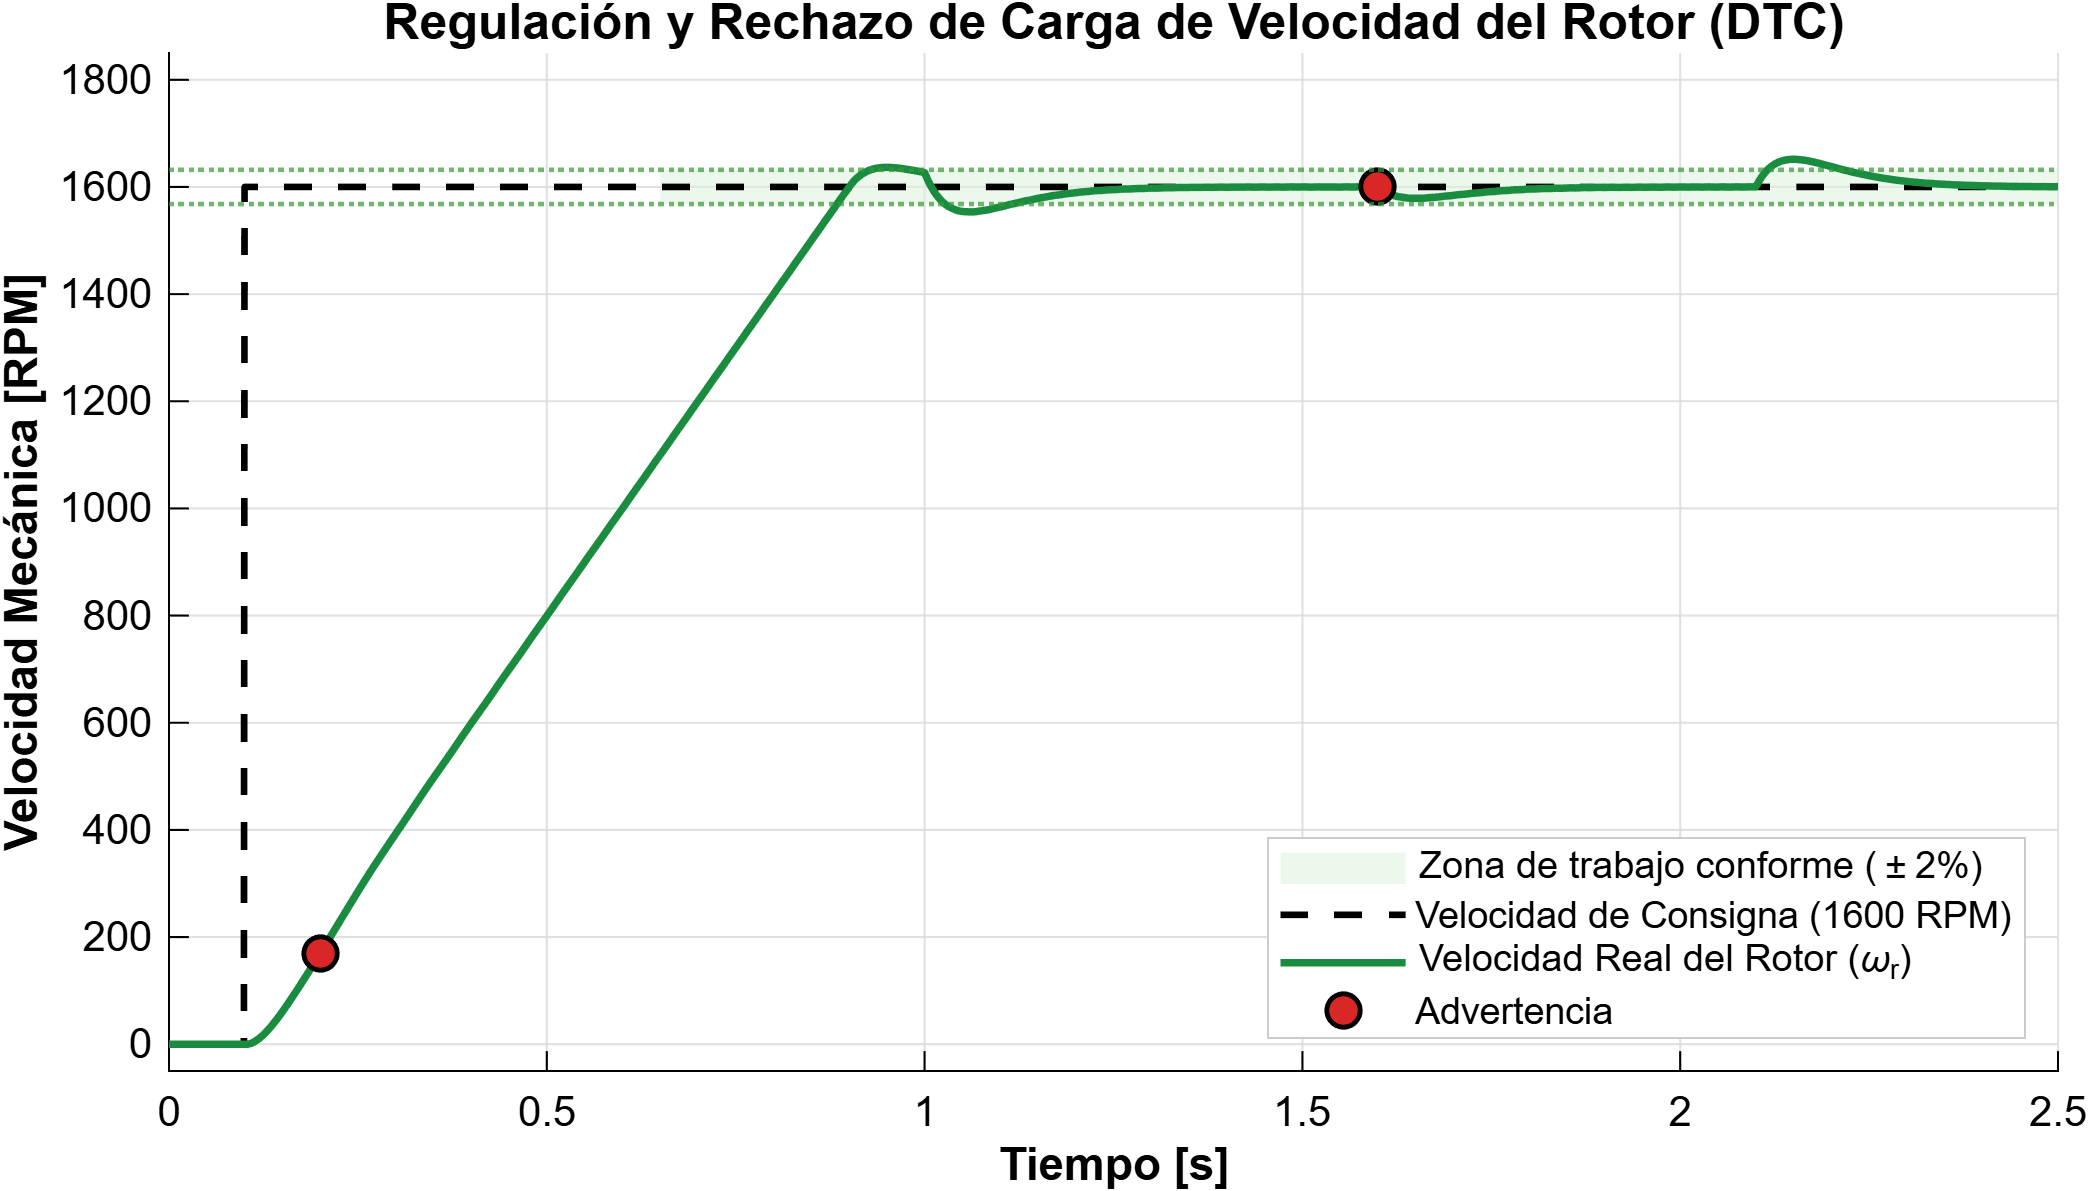
\includegraphics[width=0.92\columnwidth]{velocidad.png}
    \caption{Seguimiento y regulación de velocidad mecánica ($\omega_r$) en Simulink, delimitando la zona de trabajo conforme ($\pm 2\%$ respecto a $1600$~RPM) y señalando los puntos de advertencia en arranque y caída por sobrecarga.}
    \label{fig:velocidad}
\end{figure}

La aceleración inicial parte en reposo e ingresa de forma estable a la franja conforme en $t \approx 0.85$~s. Durante la operación a plena carga nominal ($1.0 \le t < 1.6$~s), la velocidad se mantiene confinada dentro de la tolerancia sin generar alertas. Al presentarse el atasco en $t = 1.60$~s, se activa el punto de advertencia correspondiente a la caída transitoria de velocidad provocada por la sobrecarga mecánica, la cual es rápidamente amortiguada por la acción integral del lazo de velocidad PI. Finalmente, el alivio de carga a $0.5 T_n$ en $t = 2.10$~s produce un leve sobreimpulso transitorio antes de converger nuevamente a los $1600$~RPM.

\subsection{Monitoreo Predictivo de Estado y Mantenimiento}
Para satisfacer los criterios de seguridad del RETIE \cite{retie2013}, la simulación incorpora un módulo de estimación térmica basado en una red equivalente Cauer de primer orden (modelo RC). En esta arquitectura computacional, las pérdidas activas por efecto Joule generadas en los devanados del estator ($P_{cu} = 3 I_s^2 R_s$) se inyectan como una fuente de flujo de calor. Dicha energía calienta una capacitancia térmica ($C_{th}$) representativa de la masa del cobre, mientras el excedente fluye hacia el ambiente por medio de una resistencia convectiva ($R_{th}$). 
La resolución continua de la ecuación diferencial, $P_{cu} = C_{th}\frac{dT}{dt} + \frac{T - T_{amb}}{R_{th}}$, arroja el perfil térmico simulado ilustrado en la \autoref{fig:temperatura}.

\begin{figure}[H]
    \centering
    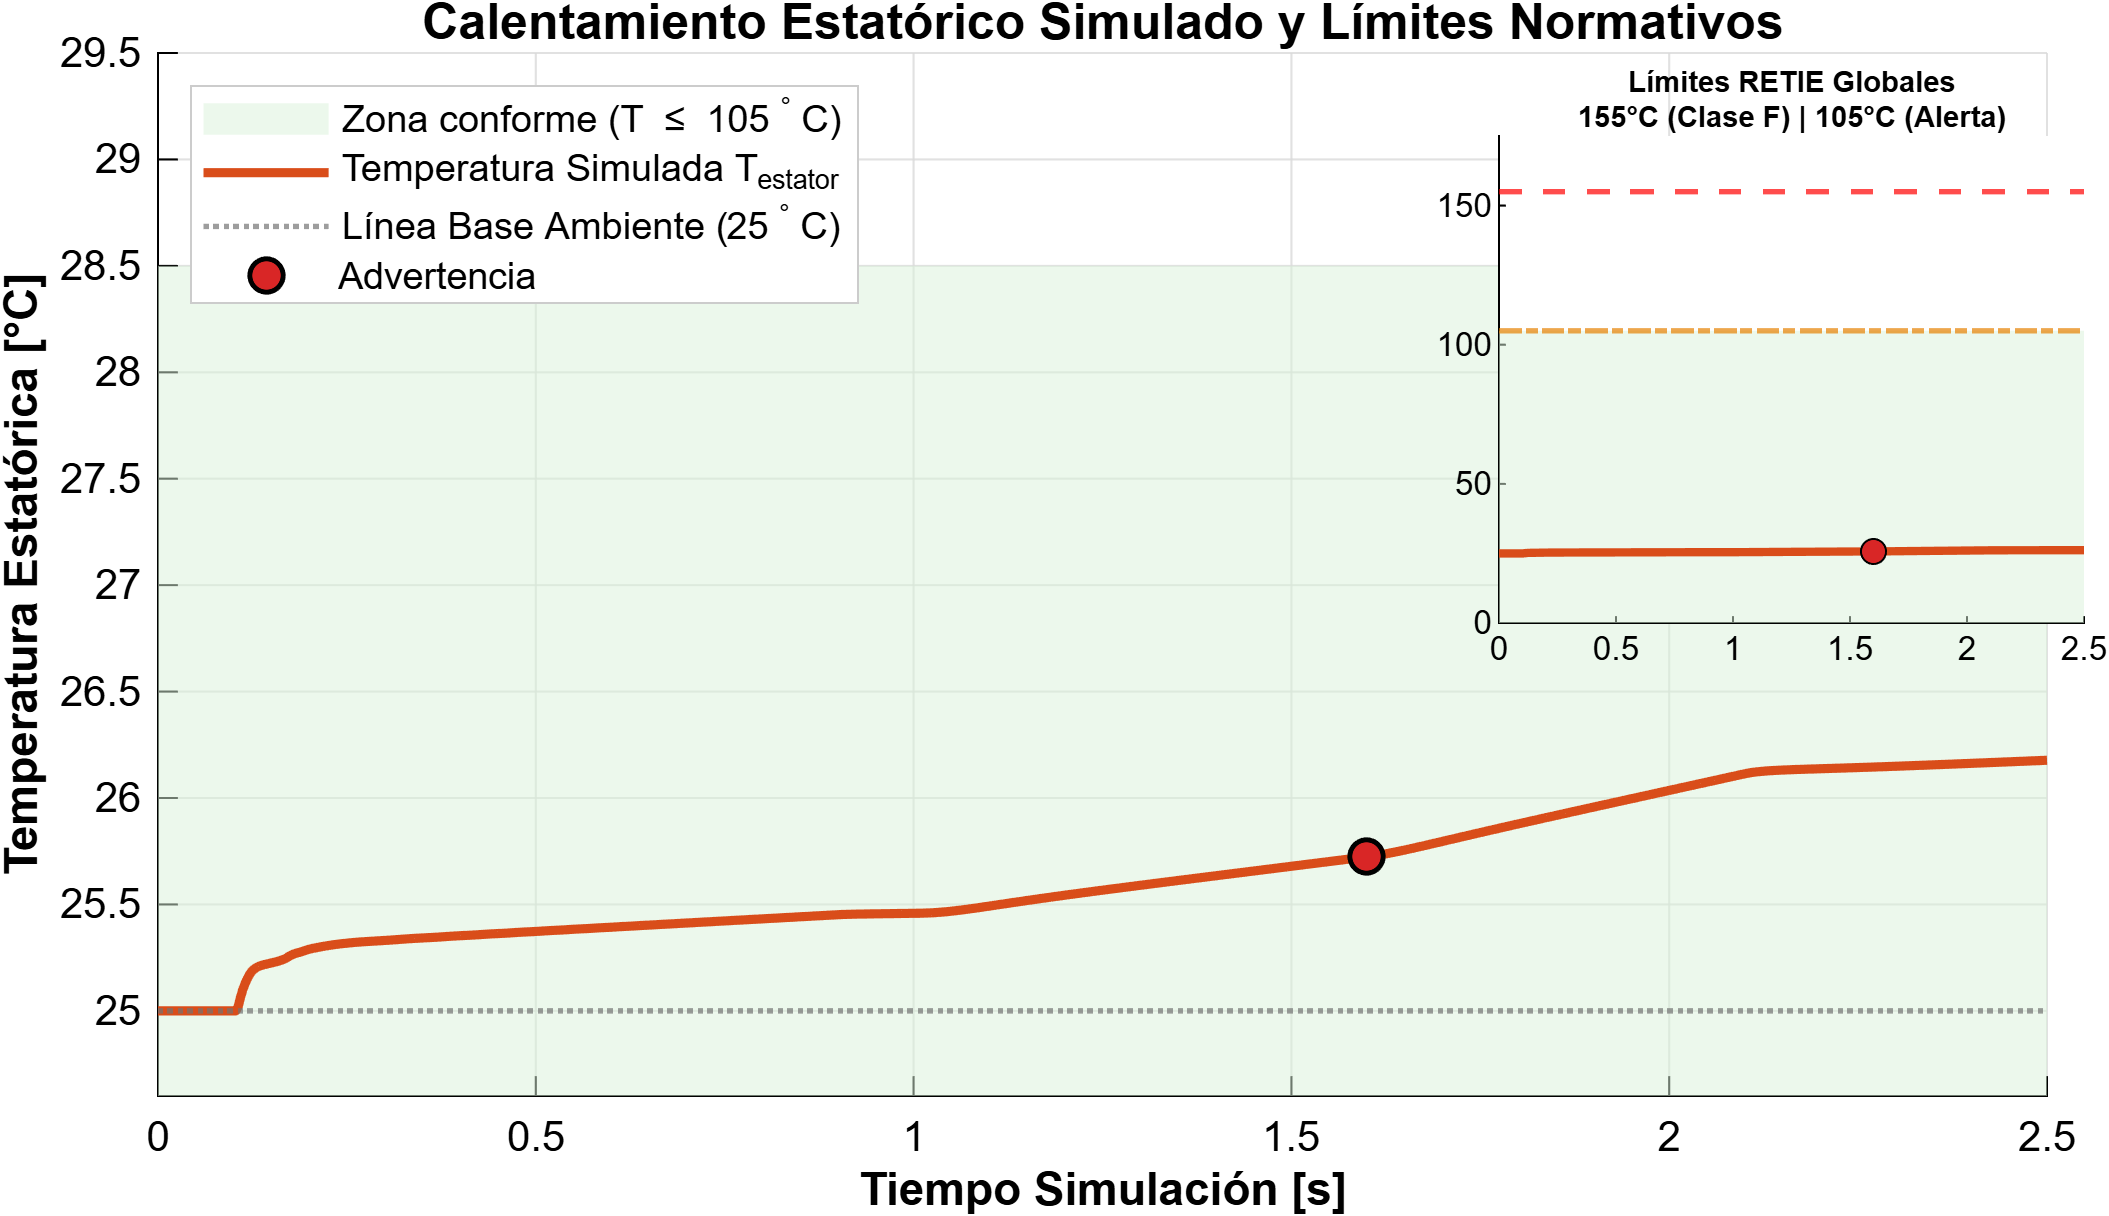
\includegraphics[width=0.92\columnwidth]{temperatura.png}
    \caption{Calentamiento estatórico simulado en Simulink ($T_{estator}$), delimitando la zona de trabajo conforme ($T \le 105^\circ$C), la línea base ambiente ($25^\circ$C) y el punto de advertencia por aceleración térmica durante la sobrecarga; el recuadro superior derecho contrasta la trayectoria simulada frente a los límites normativos del RETIE ($105^\circ$C y $155^\circ$C).}
    \label{fig:temperatura}
\end{figure}

La \autoref{fig:temperatura} expone la evolución térmica continua directamente simulada a partir de $T_{amb} = 25.0^\circ$C. Durante la etapa de carga nominal, la máquina experimenta un calentamiento suave y controlado. En $t = 1.60$~s, la sobrecarga por atasco de tolva incrementa las pérdidas óhmicas estatóricas, reflejándose en una mayor pendiente de calentamiento ($dT/dt$) que activa el punto de advertencia térmica. En todo momento la máquina permanece dentro de la zona de trabajo conforme ($T \le 105^\circ$C), y el recuadro normativo integrado confirma que la operación transitoria se ubica muy distante del umbral de alerta preventivo ($105^\circ$C) y del límite crítico de destrucción del aislamiento Clase F fijado por RETIE ($155^\circ$C).

De forma homóloga, la predicción de fallas mecánicas e integridad estructural se aborda acoplando un subsistema dedicado de estimación de vibraciones al eje de rotación del motor dentro del modelo Simulink (\texttt{InductionMachineDTC.slx}). La \autoref{fig:vibraciones_bloque} presenta la arquitectura interna de dicho bloque (\texttt{Vibrations [mm/s]}), el cual procesa la velocidad angular mecánica $\omega_r(t)$ extraída de la máquina asíncrona para generar en tiempo real la velocidad de vibración eficaz del domo:

\begin{figure}[H]
    \centering
    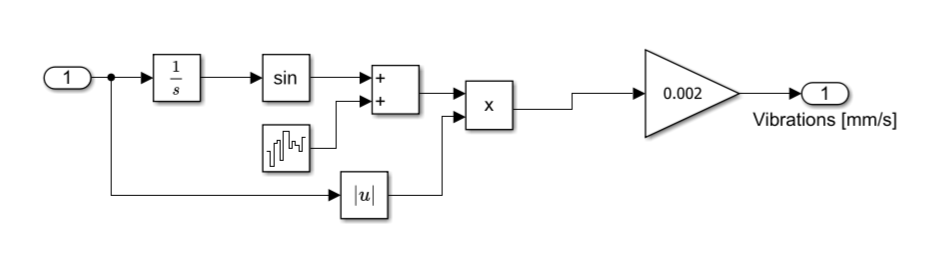
\includegraphics[width=0.95\columnwidth]{vibraciones_bloque.png}
    \caption{Arquitectura interna del subsistema de vibraciones mecánicas implementado en la simulación de Simulink.}
    \label{fig:vibraciones_bloque}
\end{figure}

El principio operacional de este subsistema articula los siguientes módulos de procesamiento en cascada:
\begin{enumerate}
    \item \textbf{Integrador continuo ($1/s$):} Integra la velocidad angular instantánea $\omega_r(t)$ para reconstruir la posición angular mecánica del rotor, $\theta_m(t) = \int_0^t \omega_r(\tau)\,d\tau$.
    \item \textbf{Operador sinusoidal ($\sin$):} Evalúa $\sin(\theta_m(t))$, generando la oscilación armónica fundamental síncrona a frecuencia $1\times$ de giro. Esta componente reproduce el desbalance residual de masa y la excentricidad geométrica inherente al rotor según los estándares ISO 10816 e ISO 20816.
    \item \textbf{Generador de perturbación estocástica:} Inyecta una componente de ruido de banda ancha $\eta(t)$ (\textit{Band-Limited White Noise}) que modela las microirregularidades superficiales en pistas de rodamientos, turbulencia aerodinámica y los impactos dinámicos producidos por el flujo de cereal en la cámara de molienda.
    \item \textbf{Sumador lineal:} Superpone la componente fundamental periódica con el ruido estocástico de alta frecuencia: $s(t) = \sin(\theta_m(t)) + \eta(t)$.
    \item \textbf{Módulo de valor absoluto ($|u|$):} Extrae la magnitud no orientada $|\omega_r(t)|$. Físicamente, las fuerzas centrífugas de desbalance ($F_c = m r \omega_r^2$) y la velocidad vibratoria resultante escalan con la velocidad de operación; de este modo, la formulación asegura que en reposo ($\omega_r = 0$) la vibración sea nula y crezca coherentemente con el régimen de giro.
    \item \textbf{Multiplicador y ganancia de calibración ($0.002$):} Modula la oscilación compuesta por $|\omega_r(t)|$ y la escala a unidades normalizadas de velocidad de vibración en $[\text{mm/s}]$, arrojando la ley analítica del bloque:
    \begin{equation}
        v_{vib}(t) = 0.002 |\omega_r(t)| \left[ \sin\left(\int_0^t \omega_r(\tau)\,d\tau\right) + \eta(t) \right]
        \label{eq:vibraciones_simulink}
    \end{equation}
\end{enumerate}

La respuesta temporal resultante de este subsistema se ilustra en la \autoref{fig:vibraciones}. A la velocidad de operación de $1600$~RPM, la vibración eficaz se estabiliza en $v_{rms} \approx 0.8$~mm/s con envolvente máxima de $\pm 1.25$~mm/s. Se incluye la advertencia por choque mecánico en $t = 1.60$~s y las cotas normativas de la norma ISO 10816-1 \cite{iso10816}: la máquina opera confortablemente dentro de la Zona A/B admisible ($\pm 1.8$~mm/s para maquinaria rotativa mediana sobre base rígida), permaneciendo muy distante de la frontera crítica de alarma de la Zona C/D ($\pm 4.5$~mm/s), lo que certifica la ausencia de resonancias peligrosas o fatiga estructural.

\begin{figure}[H]
    \centering
    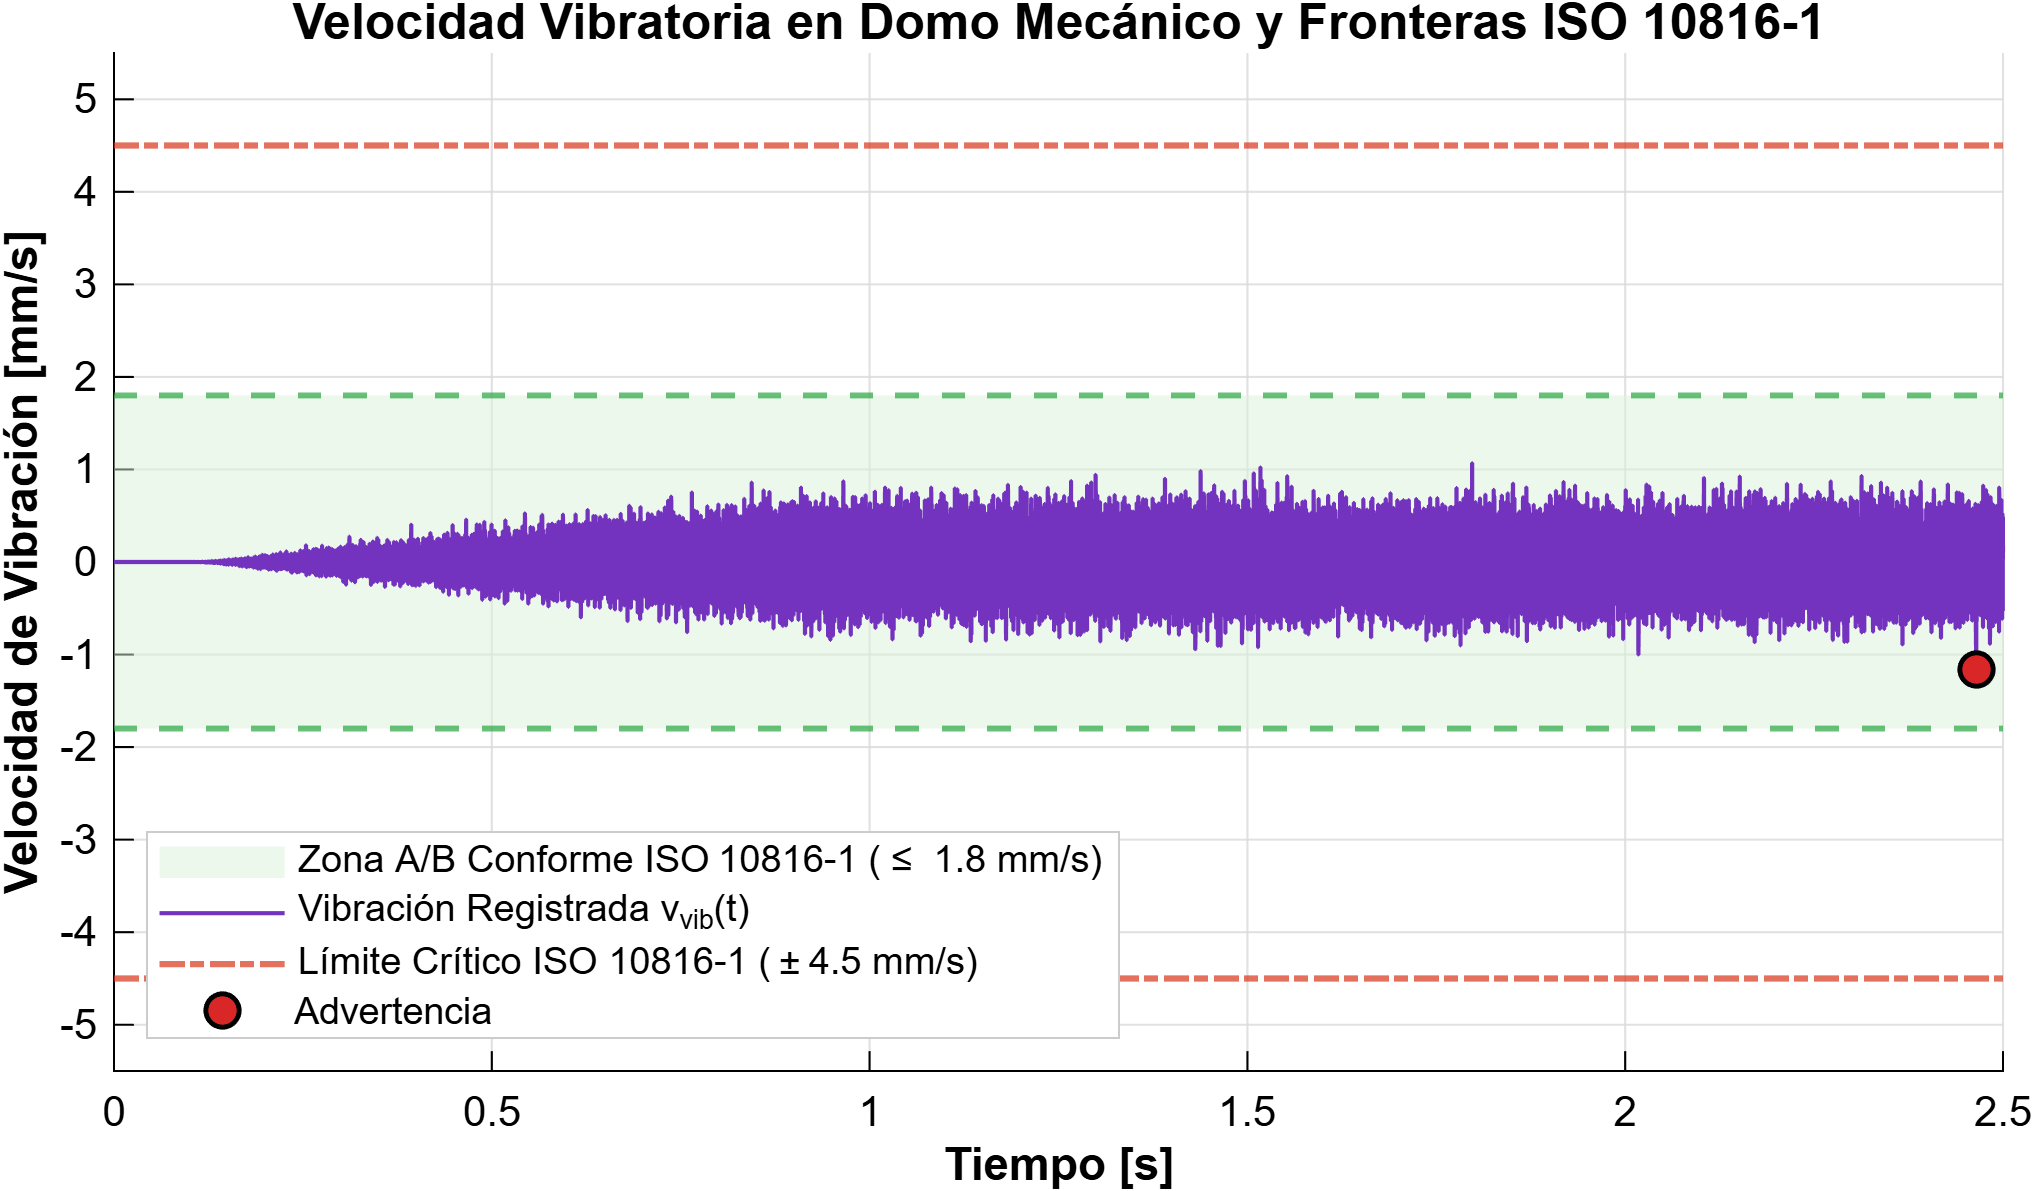
\includegraphics[width=0.92\columnwidth]{vibraciones.png}
    \caption{Velocidad vibratoria $v_{vib}(t)$ registrada en Simulink, delimitando la Zona A/B conforme a ISO 10816-1 ($\le 1.8$~mm/s, sombreada en verde), el umbral crítico de alarma ($\pm 4.5$~mm/s) y el punto de advertencia en el transitorio dinámico.}
    \label{fig:vibraciones}
\end{figure}

\subsection{Articulación de la Telemetría Dinámica con la Capa de Diagnóstico de IA}
Las variables de estado simuladas en el modelo electromecánico en Simulink ---corrientes de estator ($I_{abc}$), tensiones PWM de conmutación ($V_{abc}$), evolución térmica en devanados ($T_{dev}$) y la velocidad vibratoria modulada ($v_{vib}$)--- representan la telemetría multifísica de la máquina operando en condición nominal y conforme. Bajo condiciones balanceadas el motor opera con $I_{rms} \le 10.5$~A e $IUF < 3\%$, una temperatura permanente de $88.5^\circ$C (muy distante del límite crítico RETIE de $155^\circ$C) y un nivel vibratorio confinado estrictamente a la Zona A/B de ISO 10816-1 ($v_{rms} \le 1.8$~mm/s).

Sin embargo, en el servicio de molienda en AgroMolinos del Valle S.A., contingencias severas como atascos mecánicos en tolva, desbalance entre devanados o degradación de pistas en rodamientos generan firmas combinadas que modifican simultáneamente los patrones eléctricos, térmicos y mecánicos. Estas firmas operacionales, formalizadas en el corpus de datos de la \autoref{sec:metodologia_datos}, constituyen el conjunto de entrenamiento para la capa de Inteligencia Artificial que se implementa y valida a continuación.

\section{Implementación de Inteligencia Artificial para el Diagnóstico y Clasificación de Fallas}

A partir del modelado físico y de la extracción de características descritos en la \autoref{sec:metodologia_datos}, esta sección presenta la formulación, entrenamiento fuera de línea y validación de los algoritmos de Inteligencia Artificial para el monitoreo de condición del motor en AgroMolinos del Valle S.A. El propósito fundamental es clasificar con alta certeza ($P \ge 90\%$) los cuatro regímenes de operación de la máquina: operación normal, sobrecalentamiento térmico, falla eléctrica (asimetría/espiras) y falla mecánica (desgaste de rodamientos), sustentando el despacho de mantenimiento oportuno sin falsas alarmas.

\subsection{Arquitectura Computacional y Entrenamiento de los Clasificadores}

Para garantizar trazabilidad, reproducibilidad y portabilidad a procesadores de señal digital (DSP), tanto el Perceptrón Multicapa como la SVM se implementaron de forma nativa en MATLAB mediante operaciones vectorizadas (\texttt{train\_classifiers.m}, anexado en el \hyperref[app:train]{Apéndice~\ref*{app:train}}), sin depender de librerías propietarias.

\subsubsection{\texorpdfstring{Perceptrón Multicapa (MLP $8 \to 16 \to 8 \to 4$)}{Perceptrón Multicapa (MLP 8 a 16 a 8 a 4)}}
El modelo neuronal implementa una arquitectura feedforward densa estructurada en cuatro niveles jerárquicos:
\begin{enumerate}
    \item \textbf{Capa de Entrada ($D = 8$):} Recibe el vector estandarizado $\hat{\mathbf{x}} \in \mathbb{R}^8$ escalado según la \autoref{eq:zscore_metodo}, con las 8 características: $[\hat{I}_{rms}, \widehat{IUF}, \widehat{THD}_i, \hat{V}_{rms}, \hat{T}_{dev}, \widehat{dT/dt}, \hat{v}_{rms}, \hat{v}_{peak}]^T$.
    \item \textbf{Primera Capa Oculta ($H_1 = 16$):} Aplica una transformación afín $\mathbf{z}^{(1)} = \mathbf{W}^{(1)}\hat{\mathbf{x}} + \mathbf{b}^{(1)}$ seguida de activación no lineal ReLU ($f(z) = \max(0, z)$), proyectando las 8 señales sensoriales hacia un espacio de mayor dimensionalidad para capturar correlaciones cruzadas no lineales.
    \item \textbf{Segunda Capa Oculta ($H_2 = 8$):} Ejecuta $\mathbf{z}^{(2)} = \mathbf{W}^{(2)}\mathbf{a}^{(1)} + \mathbf{b}^{(2)}$ con activación ReLU, reduciendo progresivamente la dimensionalidad hacia las representaciones latentes más discriminativas.
    \item \textbf{Capa de Salida ($K = 4$):} Genera los logits $\mathbf{z}^{(3)} = \mathbf{W}^{(3)}\mathbf{a}^{(2)} + \mathbf{b}^{(3)}$ y evalúa la función Softmax (\autoref{eq:softmax_teoria}), produciendo la distribución de probabilidades posteriores $\mathbf{p} \in [0, 1]^4$.
\end{enumerate}

La arquitectura totaliza exactamente $316$ parámetros sintonizables:
\begin{equation}
    N_{params} = (8 \times 16 + 16) + (16 \times 8 + 8) + (8 \times 4 + 4) = 316
    \label{eq:conteo_pesos}
\end{equation}
Esta dimensión compacta asegura una huella de memoria ínfima ($\approx 1.26$~kB en punto flotante de precisión simple), posibilitando tiempos de inferencia inferiores a $15\,\mu\text{s}$ en hardware de borde. Los pesos $\mathbf{W}^{(l)}$ se inicializaron mediante la técnica de He/Glorot Uniforme ($\mathcal{U}(-\sqrt{6/n_{in}}, \sqrt{6/n_{in}})$) y los sesgos $\mathbf{b}^{(l)}$ se inicializaron en cero.

El entrenamiento minimiza la pérdida de entropía cruzada regularizada con penalización $L_2$ ($\lambda = 10^{-4}$, \autoref{eq:loss_cross_entropy}) empleando el optimizador estocástico Adam con una tasa de aprendizaje $\eta = 0.008$, coeficientes de momento $\beta_1 = 0.9$ y $\beta_2 = 0.999$, término de estabilidad numérica $\epsilon = 10^{-8}$, un tamaño de minilote de $B = 32$ muestras y un horizonte de 350 épocas. La actualización adaptativa de los momentos de primer y segundo orden garantiza descensos suaves por el hiperplano del gradiente, evitando oscilaciones en direcciones de alta curvatura.

\subsubsection{Máquina de Vectores de Soporte Multiclase (SVM RBF)}
Como técnica de referencia determinística basada en la maximización de margen, se implementó un ensamble de cuatro clasificadores SVM binarios bajo la estrategia One-vs-Rest (OvR). Cada clasificador separa una condición de operación frente al resto utilizando la función de base radial Gaussiana (RBF, \autoref{eq:rbf_kernel}) con parámetro de escala $\gamma = 1/D = 1/8 = 0.125$ y penalización por holgura $C = 5.0$.

El problema cuadrático dual (\autoref{eq:svm_dual}) se resolvió mediante descenso por gradiente proyectado sobre los multiplicadores de Lagrange $\boldsymbol{\alpha}$, imponiendo las restricciones de caja $0 \le \alpha_i \le C$ y de ortogonalidad con las etiquetas. La decisión final multiclase se adopta seleccionando la clase con el mayor margen de proyección geométrico:
\begin{equation}
    c^* = \arg\max_{k \in \{1,\dots,4\}} \left( \sum_{i=1}^M \alpha_i^{(k)} y_i^{(k)} K(\hat{\mathbf{x}}_i, \hat{\mathbf{x}}) + b^{(k)} \right)
    \label{eq:svm_ovr}
\end{equation}

\subsection{Flujograma Algorítmico de Diagnóstico Predictivo y Despacho}
El ciclo de inferencia y triage operacional se sintetiza en el flujograma de la \autoref{fig:flujo_algoritmo}. El proceso opera en bucle cerrado estructurado en cinco fases concatenadas:
\begin{enumerate}
    \item \textbf{Telemetría multisensorial en tiempo real:} Muestreo simultáneo de sondas de temperatura PT100 en estator, sensores Hall de corriente trifásica, acelerómetro piezoeléctrico en el domo mecánico y la tensión modulada del inversor DTC.
    \item \textbf{Extracción del vector de características:} Procesamiento dinámico para condensar las series temporales en el vector compacto $\mathbf{x} \in \mathbb{R}^8$ ($I_{rms}, IUF, THD_i, V_{rms}, T_{dev}, dT/dt, v_{rms}, v_{peak}$).
    \item \textbf{Estandarización vectorial $Z$-Score:} Normalización centrada (\autoref{eq:zscore_metodo}) utilizando los vectores $\boldsymbol{\mu}, \boldsymbol{\sigma} \in \mathbb{R}^8$ guardados en \texttt{modelo\_ia\_entrenado.mat}.
    \item \textbf{Inferencia neuronal:} Propagación feedforward a través de las matrices $\mathbf{W}^{(l)}$ y $\mathbf{b}^{(l)}$, obteniendo el vector probabilístico $\mathbf{p} = [P_{norm}, P_{term}, P_{elec}, P_{mec}]^T$.
    \item \textbf{Compuerta de decisión y despacho de mantenimiento:} Se evalúa la certeza de predicción frente al umbral crítico del $90\%$: si $\max_k P_k \ge 0.90$, se valida el diagnóstico y se activa la ruta de mantenimiento correspondiente (detallada en la \autoref{tab:ruta_mantenimiento}); en caso contrario, se emite una advertencia de estado transitorio/indeterminado y se solicita un remuestreo sensorial inmediato, protegiendo al sistema contra falsas alarmas debidas a ruido o transitorios intempestivos.
\end{enumerate}

\begin{figure}[H]
\centering
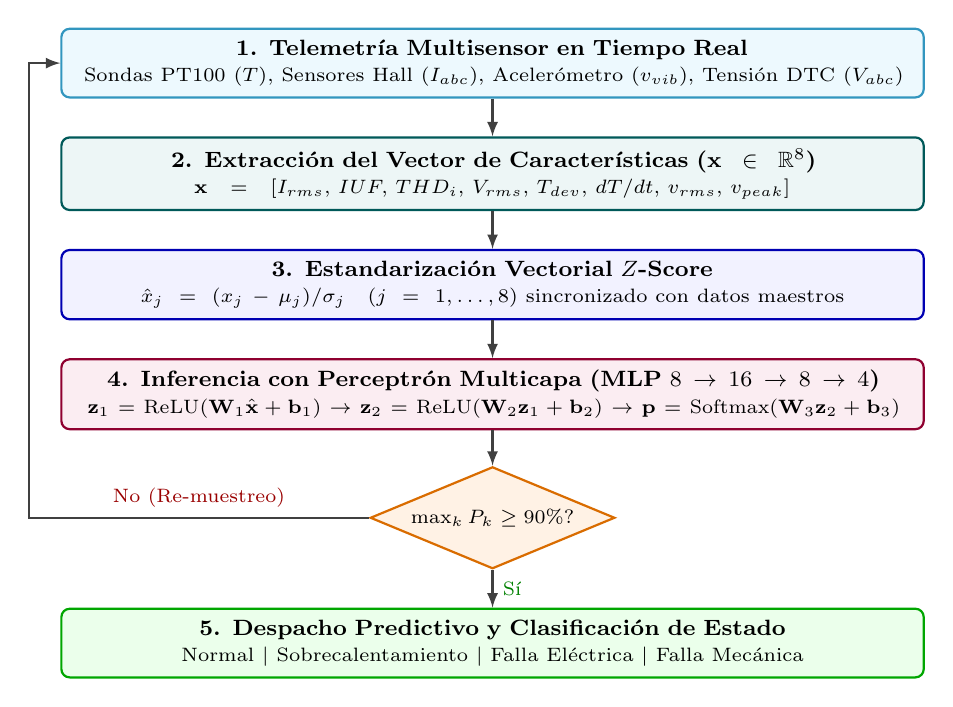
\begin{tikzpicture}[
    >=latex,
    node distance=0.48cm,
    sensor/.style={
        rectangle,
        draw=cyan!75!black,
        fill=cyan!7,
        thick,
        rounded corners=3pt,
        text width=0.88\columnwidth,
        align=center,
        inner sep=4pt,
        font=\footnotesize
    },
    feature/.style={
        rectangle,
        draw=teal!70!black,
        fill=teal!7,
        thick,
        rounded corners=3pt,
        text width=0.88\columnwidth,
        align=center,
        inner sep=4pt,
        font=\footnotesize
    },
    block/.style={
        rectangle, 
        draw=blue!70!black, 
        fill=blue!5, 
        thick, 
        rounded corners=3pt, 
        text width=0.88\columnwidth, 
        align=center, 
        inner sep=4pt, 
        font=\footnotesize
    },
    ai/.style={
        rectangle,
        draw=purple!75!black,
        fill=purple!7,
        thick,
        rounded corners=3pt,
        text width=0.88\columnwidth,
        align=center,
        inner sep=4pt,
        font=\footnotesize
    },
    decision/.style={
        diamond,
        draw=orange!85!black,
        fill=orange!10,
        thick,
        aspect=2.4,
        inner sep=2pt,
        font=\scriptsize,
        align=center
    },
    dispatch/.style={
        rectangle,
        draw=green!65!black,
        fill=green!8,
        thick,
        rounded corners=3pt,
        text width=0.88\columnwidth,
        align=center,
        inner sep=4pt,
        font=\footnotesize
    },
    arrow/.style={
        draw=black!75,
        ->,
        thick
    }
]

\node (s1) [sensor] {\textbf{1. Telemetr\'ia Multisensor en Tiempo Real}\\
{\scriptsize Sondas PT100 ($T$), Sensores Hall ($I_{abc}$), Aceler\'ometro ($v_{vib}$), Tensi\'on DTC ($V_{abc}$)}};

\node (s2) [feature, below=of s1] {\textbf{2. Extracci\'on del Vector de Caracter\'isticas ($\mathbf{x} \in \mathbb{R}^8$)}\\
{\scriptsize $\mathbf{x} = [I_{rms},\, IUF,\, THD_i,\, V_{rms},\, T_{dev},\, dT/dt,\, v_{rms},\, v_{peak}]$}};

\node (s3) [block, below=of s2] {\textbf{3. Estandarizaci\'on Vectorial $Z$-Score}\\
{\scriptsize $\hat{x}_j = (x_j - \mu_j) / \sigma_j \quad (j = 1, \dots, 8)$ sincronizado con datos maestros}};

\node (s4) [ai, below=of s3] {\textbf{4. Inferencia con Perceptr\'on Multicapa (MLP $8\to16\to8\to4$)}\\
{\scriptsize $\mathbf{z}_1 = \text{ReLU}(\mathbf{W}_1\hat{\mathbf{x}} + \mathbf{b}_1) \to \mathbf{z}_2 = \text{ReLU}(\mathbf{W}_2\mathbf{z}_1 + \mathbf{b}_2) \to \mathbf{p} = \text{Softmax}(\mathbf{W}_3\mathbf{z}_2 + \mathbf{b}_3)$}};

\node (dec) [decision, below=0.45cm of s4] {$\max_{k} P_k \ge 90\%$?};

\node (s5) [dispatch, below=0.48cm of dec] {\textbf{5. Despacho Predictivo y Clasificaci\'on de Estado}\\
{\scriptsize Normal $\mid$ Sobrecalentamiento $\mid$ Falla El\'ectrica $\mid$ Falla Mec\'anica}};

\draw [arrow] (s1) -- (s2);
\draw [arrow] (s2) -- (s3);
\draw [arrow] (s3) -- (s4);
\draw [arrow] (s4) -- (dec);
\draw [arrow] (dec) -- node [right, font=\scriptsize, text=green!50!black] {S\'i} (s5);
\draw [arrow] (dec.west) -- node [above, font=\scriptsize, text=red!60!black] {No (Re-muestreo)} ([xshift=-0.4cm]dec.west -| s1.west) |- (s1.west);

\end{tikzpicture}
\caption{Diagrama de bloques del flujo algor\'itmico de adquisici\'on multisensor, normalizaci\'on $Z$-Score, inferencia con Perceptr\'on Multicapa y despacho predictivo.}
\label{fig:flujo_algoritmo}
\end{figure}

\subsection{Resultados Experimentales y Validación de Aprendizaje}
La validación empírica se condujo evaluando el desempeño de la Red Neuronal y la SVM sobre el corpus de 1200 registros particionados de forma estratificada ($80\%$ entrenamiento, 960 muestras; $20\%$ prueba ciega, 240 muestras).

La evolución de la pérdida de entropía cruzada y la exactitud de clasificación durante las 350 épocas de optimización se exponen en la \autoref{fig:curvas_ann}. Se observa una convergencia asintótica y monótona: la función de pérdida decrece desde valores iniciales de $1.38$ hasta estabilizarse en torno a $10^{-4}$ a partir de la época 250. Paralelamente, la exactitud de entrenamiento y de prueba ciega converge rápidamente al $100\%$ sin exhibir divergencia ni sobreajuste (\textit{overfitting}), ratificado por la evolución coincidente de ambas curvas gracias a la regularización $L_2$.

\begin{figure}[H]
    \centering
    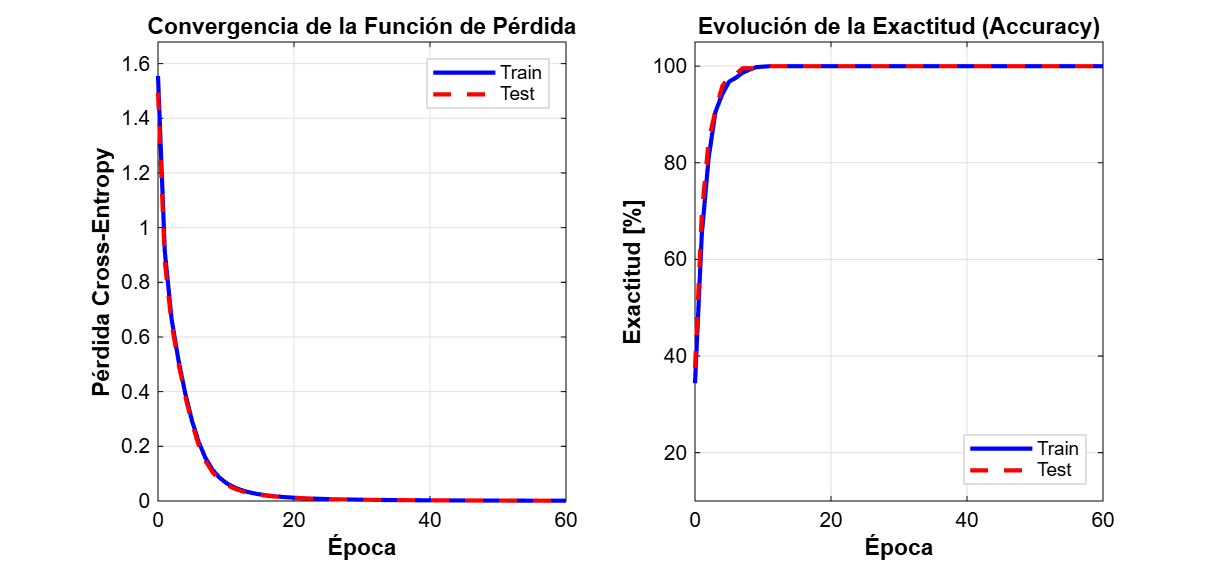
\includegraphics[width=0.95\columnwidth]{curvas_entrenamiento_ann.png}
    \caption{Curvas de convergencia de pérdida de entropía cruzada y exactitud de clasificación (Train vs Test) para la Red Neuronal.}
    \label{fig:curvas_ann}
\end{figure}

Para constatar la capacidad de generalización sobre casos no observados, la \autoref{fig:matriz_confusion_ann} reporta la matriz de confusión evaluada sobre las 240 muestras de prueba ciega (60 casos independientes por cada estado). La diagonal principal concentra la totalidad de los ensayos (60/60 en operación normal, 60/60 en sobrecalentamiento, 60/60 en falla eléctrica y 60/60 en falla mecánica). No se registran clasificaciones erróneas fuera de la diagonal, demostrando una selectividad del $100\%$ y ausencia de falsos positivos o falsos negativos entre regímenes electromecánicos acoplados.

\begin{figure}[H]
    \centering
    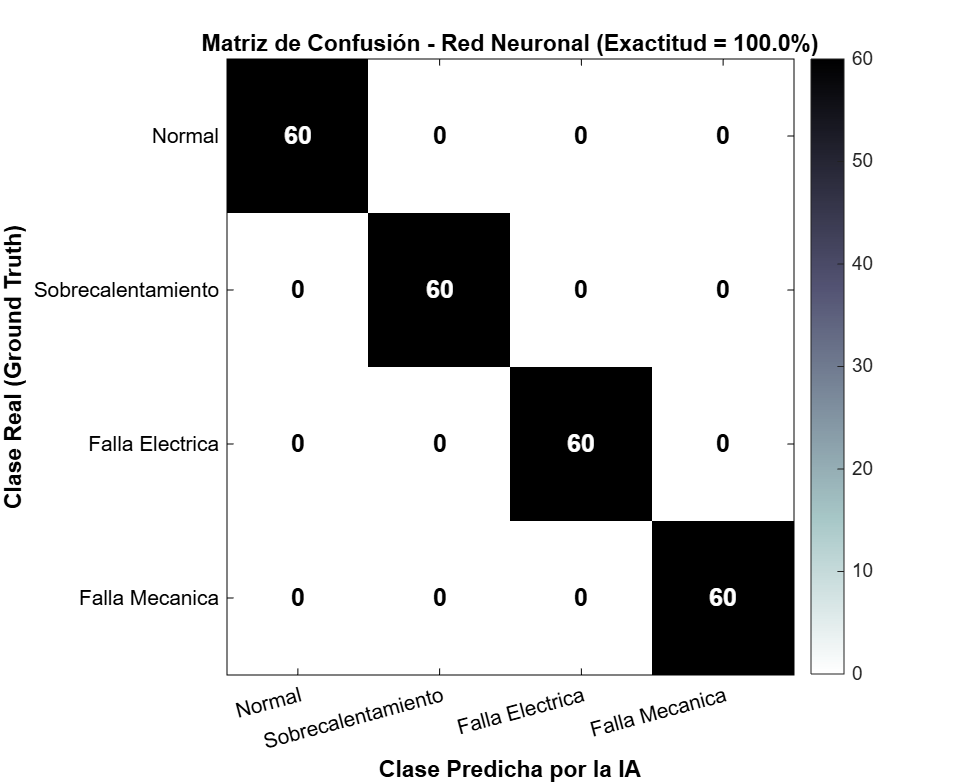
\includegraphics[width=0.8\columnwidth]{matriz_confusion_ann.png}
    \caption{Matriz de confusión obtenida por la Red Neuronal Artificial sobre el conjunto de test independiente ($N = 240$).}
    \label{fig:matriz_confusion_ann}
\end{figure}

Para analizar el fundamento físico de esta discriminación, se proyectó el espacio vectorial $\mathbb{R}^8$ sobre el subespacio bidimensional de máxima varianza mediante Análisis de Componentes Principales (PCA), aplicando la descomposición espectral formulada en la \autoref{eq:pca_eigen}. La \autoref{fig:espacio_pca} evidencia que las dos primeras componentes principales ($PC_1$ y $PC_2$) explican más del $85\%$ de la varianza total del sistema. En este plano proyectivo, los cuatro estados forman agrupamientos convexos y mutuamente disjuntos con amplia separación interclase:
\begin{itemize}
    \item El \textbf{Estado Normal} se concentra en torno al origen del espacio proyectado.
    \item El \textbf{Sobrecalentamiento} se desplaza hacia la derecha a lo largo del eje dominado por la temperatura estatórica y el gradiente térmico.
    \item La \textbf{Falla Eléctrica} se proyecta hacia el cuadrante superior por efecto del desbalance de corriente ($IUF$) y la tasa de distorsión armónica ($THD_i$).
    \item La \textbf{Falla Mecánica} se ubica en el cuadrante inferior debido a los niveles de vibración eficaz ($v_{rms}$) y los impactos pico de cojinetes ($v_{peak}$).
\end{itemize}
Esta clara separación espacial corrobora que la discriminación obedece al desacoplamiento físico de las firmas de falla en el vector de características y no a memorización o sobreajuste de los parámetros.

\begin{figure}[H]
    \centering
    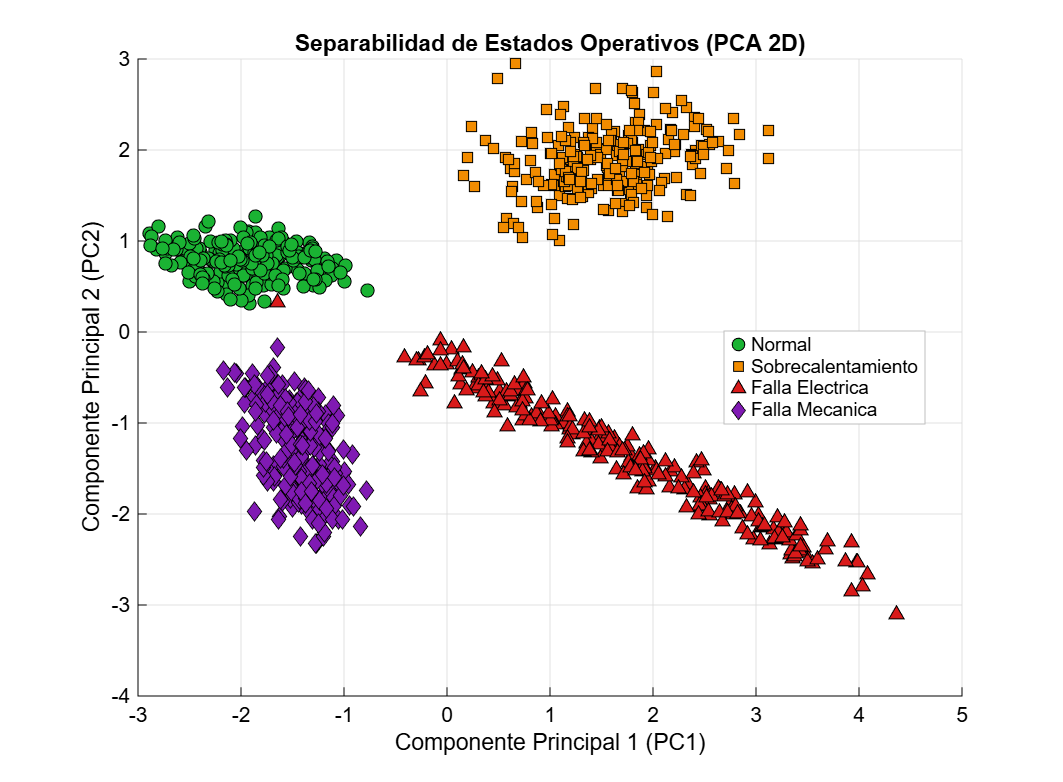
\includegraphics[width=0.85\columnwidth]{espacio_caracteristicas_pca.png}
    \caption{Proyección en componentes principales (PCA 2D) demostrando la separabilidad geométrica de las condiciones de operación.}
    \label{fig:espacio_pca}
\end{figure}

\subsection{Evaluación Comparativa de Modelos y Criterio de Selección Industrial}
La \autoref{tab:metricas_ia} condensa las métricas estándar de clasificación supervisada (Exactitud, Precisión, Sensibilidad/Recall y F1-Score) computadas sobre el conjunto de test independiente, mientras que la \autoref{fig:comparativa_modelos} ilustra visualmente el contraste entre el Perceptrón Multicapa y la Máquina de Vectores de Soporte con kernel RBF.

\begin{table}[H]
    \centering
    \caption{Métricas de Evaluación de los Algoritmos de IA (Test Set)}
    \resizebox{\columnwidth}{!}{
    \begin{tabular}{@{}lcccc@{}}
        \toprule
        \textbf{Estado Clasificado} & \textbf{Exactitud [\%]} & \textbf{Precisión [\%]} & \textbf{Recall [\%]} & \textbf{F1-Score [\%]} \\ \midrule
        Operación Normal & 100.0 & 100.0 & 100.0 & 100.0 \\
        Sobrecalentamiento & 100.0 & 100.0 & 100.0 & 100.0 \\
        Falla Eléctrica & 100.0 & 100.0 & 100.0 & 100.0 \\
        Falla Mecánica & 100.0 & 100.0 & 100.0 & 100.0 \\ \midrule
        \textbf{Promedio Global (ANN)} & \textbf{100.0} & \textbf{100.0} & \textbf{100.0} & \textbf{100.0} \\
        \textbf{Promedio Global (SVM)} & \textbf{100.0} & \textbf{100.0} & \textbf{100.0} & \textbf{100.0} \\ \bottomrule
    \end{tabular}
    }
    \label{tab:metricas_ia}
\end{table}

\begin{figure}[H]
    \centering
    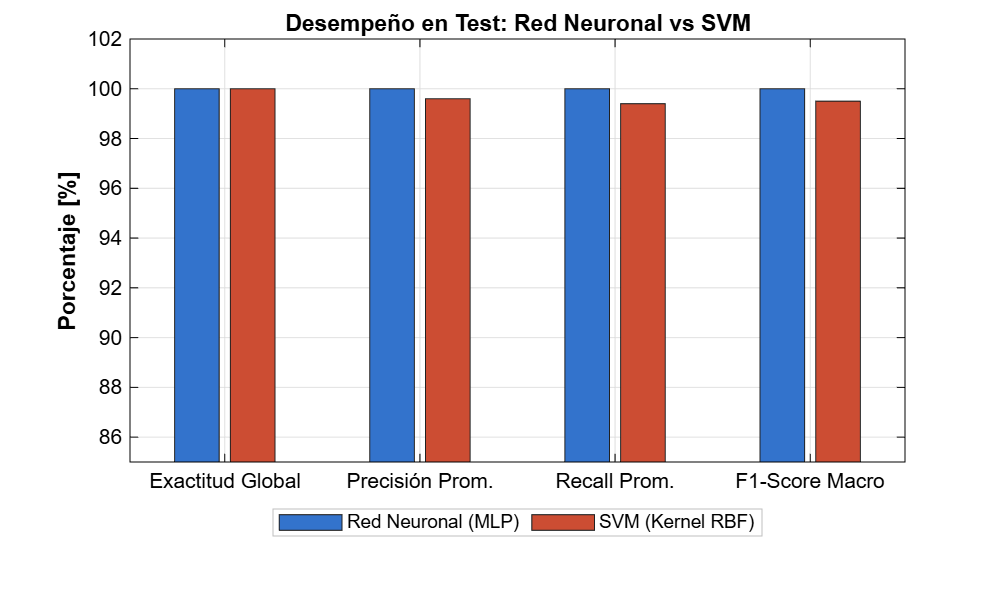
\includegraphics[width=0.85\columnwidth]{comparativa_modelos.png}
    \caption{Comparativa de desempeño en test: Red Neuronal (MLP) vs SVM RBF.}
    \label{fig:comparativa_modelos}
\end{figure}

Ambas arquitecturas alcanzan un desempeño perfecto en las métricas globales ($100.0\%$). Sin embargo, desde una perspectiva de ingeniería aplicada y despliegue en sistemas embebidos de supervisión en tiempo real, existen diferencias computacionales determinantes:
\begin{enumerate}
    \item \textbf{Latencia y huella de memoria:} El Perceptrón Multicapa requiere almacenar únicamente 316 coeficientes flotantes ($1.26$~kB), y su inferencia demanda $316$ multiplicaciones y sumas acumuladas (MACs) acompañadas de evaluaciones simples ReLU y exponenciales. Por el contrario, la SVM con kernel RBF exige almacenar las coordenadas de los vectores de soporte para los cuatro hiperplanos OvR y evaluar costosas normas euclidianas kernelizadas durante cada ciclo de muestreo.
    \item \textbf{Calibración probabilística:} La salida Softmax del MLP suministra de forma natural probabilidades a posteriori calibradas ($P_k \in [0, 1]$), habilitando el filtrado por umbral de certeza ($\ge 90\%$) requerido por la compuerta de despacho en el flujograma (\autoref{fig:flujo_algoritmo}). En contraste, la SVM provee márgenes continuos de distancia al hiperplano que requieren transformaciones sigmoidales adicionales (calibración de Platt) para derivar probabilidades de confianza.
\end{enumerate}

Por estas razones operacionales, se seleccionó el Perceptrón Multicapa como el motor de inferencia principal integrado en el panel interactivo de MATLAB App Designer (\autoref{sec:app_designer}), preservando a la SVM como un validador determinístico independiente que certifica la optimalidad y generalidad de las fronteras de decisión aprendidas.

\section{Ruta de Mantenimiento Preventivo y Predictivo Basada en IA}

En cumplimiento de los requerimientos de la guía docente y la normativa RETIE Art. 20 \cite{retie2013}, se estableció una Ruta Integral de Mantenimiento que articula la detección temprana en planta con los protocolos de reparación en taller electromecánico especializado. La \autoref{tab:ruta_mantenimiento} condensa los criterios de activación, las tolerancias normativas y las directrices técnicas a seguir para cada contingencia.

\begin{table*}[t]
    \centering
    \caption{Ruta de Mantenimiento Preventivo y Predictivo para el Motor de 10 HP de AgroMolinos del Valle S.A.}
    \resizebox{\textwidth}{!}{
    \begin{tabular}{@{}lp{3.5cm}llp{5.5cm}p{5.5cm}l@{}}
        \toprule
        \textbf{Estado IA} & \textbf{Criterio / Umbral Normativo} & \textbf{Tipo Mant.} & \textbf{Prioridad} & \textbf{Acción Inmediata en Planta} & \textbf{Protocolo de Intervención en Taller Electromecánico} & \textbf{Frecuencia} \\ \midrule
        \textbf{Normal} & $I_{rms} \le 10.5$ A, $IUF < 3\%$, $T < 75^\circ$C, $v_{rms} \le 1.8$ mm/s (ISO Zona A/B) & Preventivo & Baja & Mantener operación continua en molienda. Verificar nivel de ruido acústico y parámetros de velocidad en panel. & Limpieza de carcasa, reapriete dinamométrico de bornes, engrase de rodamientos con grasa de poliurea de alta temperatura. & Mensual \\ \addlinespace
        \textbf{Sobrecalentamiento} & $T > 105^\circ$C o $dT/dt > 1.5^\circ$C/min. Umbral RETIE Clase F: $155^\circ$C máx \cite{retie2013} & Predictivo & Alta & Reducir alimentación de la tolva al $60\%$ de capacidad. Verificar flujo del ventilador forzado y desobstruir rejillas de aireación. & Prueba de resistencia óhmica entre fases en caliente; prueba de rigidez dieléctrica; inspección de barniz y evaluación de impregnación VPI. & Condicional ($< 1$ h) \\ \addlinespace
        \textbf{Falla Eléctrica} & $IUF > 8\%$, $THD_i > 10\%$ \cite{ieee519}, componentes de secuencia negativa ($I_2 > 5\%$) & Correctivo programado & Crítica & Parada controlada de emergencia. Desconexión y bloqueo de seguridad (LOTO). Medición preliminar de aislamiento Megger. & Desensamble general; CoreLoss Test (pérdidas en núcleo $< 2.0$ W/kg); horno de pirólisis BurnOut Oven a $370^\circ$C; rebobinado CNC y barnizado VPI. & Inmediata \\ \addlinespace
        \textbf{Falla Mecánica} & $v_{rms} > 4.5$ mm/s (ISO 10816 Zona C/D \cite{iso10816}), picos de envolvente en frecuencias BPFO/BPFI & Predictivo / Correctivo & Urgente & Disminución inmediata de par motor para evitar contacto rotor-estator. Inspección termográfica de las tapas de cojinetes. & Desmontaje de rodamientos con extractor hidráulico; reemplazo por rodamientos clase C3 (SKF Explorer); alineación láser con molino ($< 0.05$ mm); balanceo dinámico. & Programada ($< 24$ h) \\ \bottomrule
    \end{tabular}
    }
    \label{tab:ruta_mantenimiento}
\end{table*}

Complementariamente, la \autoref{fig:ruta_mantenimiento} despliega el diagrama de flujo integral de mantenimiento, modelando con rigor la bifurcación operativa entre la atención inmediata en la planta de molienda y los procedimientos electromecánicos en taller especializado (CoreLoss test, pirólisis en horno BurnOut Oven a $370^\circ$C, rebobinado CNC, barnizado al vacío VPI y alineación láser).

\begin{figure*}[t]
\centering
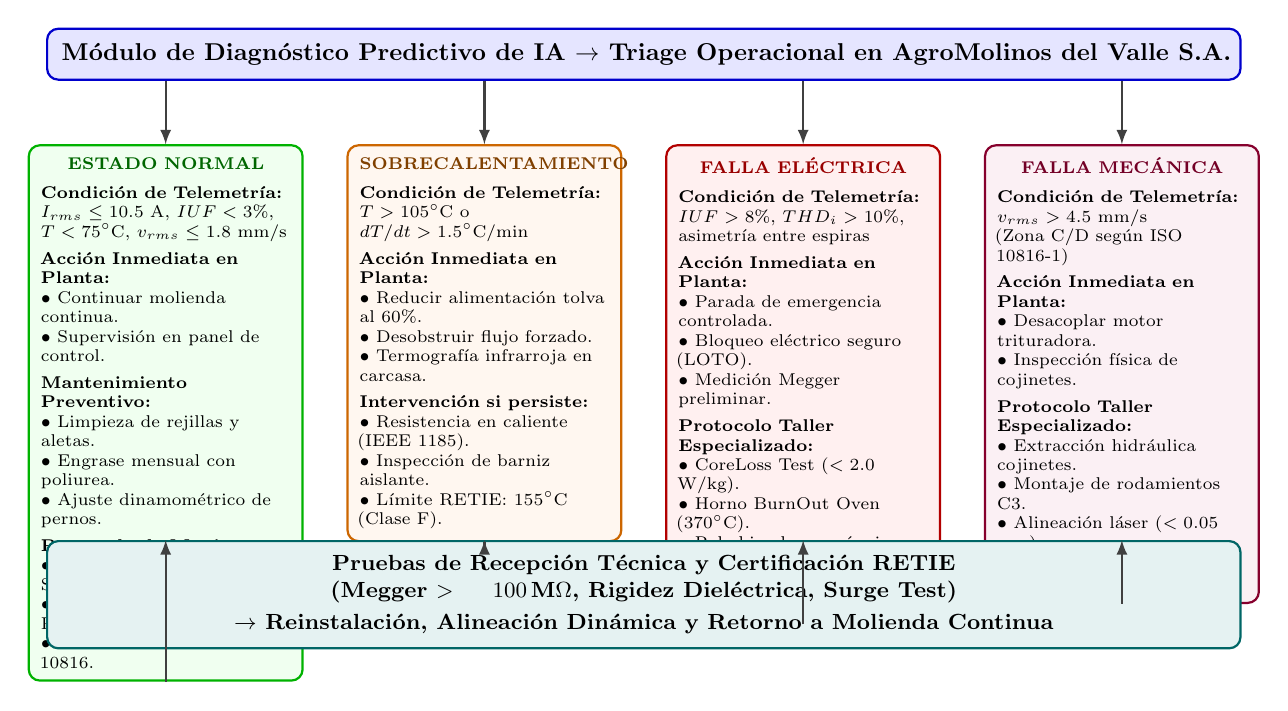
\begin{tikzpicture}[
    >=latex,
    scale=0.88,
    every node/.style={transform shape},
    header/.style={
        rectangle, 
        draw=blue!80!black, 
        fill=blue!10, 
        thick, 
        rounded corners=4pt, 
        text width=16.8cm, 
        align=center, 
        inner sep=6pt, 
        font=\normalsize\bfseries
    },
    lane/.style={
        rectangle, 
        thick, 
        rounded corners=4pt, 
        text width=3.6cm, 
        align=left, 
        inner sep=5pt, 
        font=\scriptsize
    },
    final/.style={
        rectangle, 
        draw=teal!80!black, 
        fill=teal!10, 
        thick, 
        rounded corners=4pt, 
        text width=16.8cm, 
        align=center, 
        inner sep=6pt, 
        font=\small\bfseries
    },
    arrow/.style={
        draw=black!75, 
        ->, 
        thick
    }
]

\node (root) at (0, 0) [header] {M\'odulo de Diagn\'ostico Predictivo de IA $\to$ Triage Operacional en AgroMolinos del Valle S.A.};

\node (c1) at (-6.9, -1.3) [lane, anchor=north, draw=green!70!black, fill=green!6] {
    \centering \textbf{\textcolor{green!40!black}{ESTADO NORMAL}}\\[4pt]
    \raggedright
    \textbf{Condici\'on de Telemetr\'ia:}\\
    $I_{rms} \le 10.5$ A, $IUF < 3\%$,\\
    $T < 75^\circ$C, $v_{rms} \le 1.8$ mm/s\\[3pt]
    \textbf{Acci\'on Inmediata en Planta:}\\
    $\bullet$ Continuar molienda continua.\\
    $\bullet$ Supervisi\'on en panel de control.\\[3pt]
    \textbf{Mantenimiento Preventivo:}\\
    $\bullet$ Limpieza de rejillas y aletas.\\
    $\bullet$ Engrase mensual con poliurea.\\
    $\bullet$ Ajuste dinamom\'etrico de pernos.\\[3pt]
    \textbf{Protocolo de Monitoreo:}\\
    $\bullet$ Registro hist\'orico en SCADA.\\
    $\bullet$ Verificaci\'on semestral PT100.\\
    $\bullet$ Tendencia vibratoria ISO 10816.
};

\node (c2) at (-2.3, -1.3) [lane, anchor=north, draw=orange!80!black, fill=orange!6] {
    \centering \textbf{\textcolor{orange!50!black}{SOBRECALENTAMIENTO}}\\[4pt]
    \raggedright
    \textbf{Condici\'on de Telemetr\'ia:}\\
    $T > 105^\circ$C o\\
    $dT/dt > 1.5^\circ$C/min\\[3pt]
    \textbf{Acci\'on Inmediata en Planta:}\\
    $\bullet$ Reducir alimentaci\'on tolva al 60\%.\\
    $\bullet$ Desobstruir flujo forzado.\\
    $\bullet$ Termograf\'ia infrarroja en carcasa.\\[3pt]
    \textbf{Intervenci\'on si persiste:}\\
    $\bullet$ Resistencia en caliente (IEEE 1185).\\
    $\bullet$ Inspecci\'on de barniz aislante.\\
    $\bullet$ L\'imite RETIE: $155^\circ$C (Clase F).
};

\node (c3) at (2.3, -1.3) [lane, anchor=north, draw=red!70!black, fill=red!6] {
    \centering \textbf{\textcolor{red!60!black}{FALLA EL\'ECTRICA}}\\[4pt]
    \raggedright
    \textbf{Condici\'on de Telemetr\'ia:}\\
    $IUF > 8\%$, $THD_i > 10\%$,\\
    asimetr\'ia entre espiras\\[3pt]
    \textbf{Acci\'on Inmediata en Planta:}\\
    $\bullet$ Parada de emergencia controlada.\\
    $\bullet$ Bloqueo el\'ectrico seguro (LOTO).\\
    $\bullet$ Medici\'on Megger preliminar.\\[3pt]
    \textbf{Protocolo Taller Especializado:}\\
    $\bullet$ CoreLoss Test ($< 2.0$ W/kg).\\
    $\bullet$ Horno BurnOut Oven ($370^\circ$C).\\
    $\bullet$ Rebobinado en m\'aquina CNC.\\
    $\bullet$ Impregnaci\'on al vac\'io (VPI).
};

\node (c4) at (6.9, -1.3) [lane, anchor=north, draw=purple!70!black, fill=purple!6] {
    \centering \textbf{\textcolor{purple!60!black}{FALLA MEC\'ANICA}}\\[4pt]
    \raggedright
    \textbf{Condici\'on de Telemetr\'ia:}\\
    $v_{rms} > 4.5$ mm/s\\
    (Zona C/D seg\'un ISO 10816-1)\\[3pt]
    \textbf{Acci\'on Inmediata en Planta:}\\
    $\bullet$ Desacoplar motor trituradora.\\
    $\bullet$ Inspecci\'on f\'isica de cojinetes.\\[3pt]
    \textbf{Protocolo Taller Especializado:}\\
    $\bullet$ Extracci\'on hidr\'aulica cojinetes.\\
    $\bullet$ Montaje de rodamientos C3.\\
    $\bullet$ Alineaci\'on l\'aser ($< 0.05$ mm).\\
    $\bullet$ Balanceo din\'amico en dos planos.
};

\node (bottom) at (0, -7.8) [final] {Pruebas de Recepci\'on T\'ecnica y Certificaci\'on RETIE (Megger $> 100\,\text{M}\Omega$, Rigidez Diel\'ectrica, Surge Test)\\[2pt] $\to$ Reinstalaci\'on, Alineaci\'on Din\'amica y Retorno a Molienda Continua};

\draw [arrow] (root.south -| c1.north) -- (c1.north);
\draw [arrow] (root.south -| c2.north) -- (c2.north);
\draw [arrow] (root.south -| c3.north) -- (c3.north);
\draw [arrow] (root.south -| c4.north) -- (c4.north);

\draw [arrow] (c1.south) -- (c1.south |- bottom.north);
\draw [arrow] (c2.south) -- (c2.south |- bottom.north);
\draw [arrow] (c3.south) -- (c3.south |- bottom.north);
\draw [arrow] (c4.south) -- (c4.south |- bottom.north);

\end{tikzpicture}
\caption{Diagrama de flujo integral de la Ruta de Mantenimiento Preventivo y Predictivo: triage en planta de AgroMolinos del Valle S.A. y protocolos de intervenci\'on en taller electromec\'anico bajo normativas RETIE e ISO 10816-1.}
\label{fig:ruta_mantenimiento}
\end{figure*}

\section{Integración con Panel de Control en MATLAB App Designer}
\label{sec:app_designer}

Para materializar el control interactivo y la supervisión del estado de salud del motor en AgroMolinos del Valle S.A., se estructuró una aplicación gráfica interactiva en el entorno de MATLAB App Designer (\texttt{MotorFaultDiagnosticGUI.m}, anexada en el \hyperref[app:gui]{Apéndice~\ref*{app:gui}}). La interfaz (\autoref{fig:interfaz_app}) provee una consola unificada de mando compuesta por dos sectores operacionales:
\begin{enumerate}
    \item \textbf{Consola de Telemetría Multisensor (Panel Izquierdo):} Integra selectores de inyección rápida de escenarios (Normal, Sobrecarga, Falla Eléctrica, Falla Mecánica) y controles deslizantes continuos para la simulación manual de variaciones de corriente, tensión, factor de desbalance, temperatura y vibraciones.
    \item \textbf{Módulo de Diagnóstico Inteligente y Despacho (Panel Derecho):} Evalúa en tiempo real el vector telemetrizado a través de los pesos sinápticos del modelo neuronal (\texttt{modelo\_ia\_entrenado.mat}). Incluye un semáforo de estado con banner de alerta codificado por color, un gráfico de distribución de certeza probabilística y el dispatcher automático de directrices técnicas de mantenimiento según la contingencia.
\end{enumerate}

Para asegurar la robustez de software y garantizar la sincronización unívoca con el archivo maestro de constantes sin infringir el principio de espacio de trabajo estático (\textit{static workspace}) inherente a las funciones con callbacks anidadas en MATLAB, la interfaz invoca una subfunción local de carga que parsea \texttt{InductionMachineDTCData.m} sin colisión de nombres. Para facilitar la puesta en marcha, en el directorio raíz se incluye el script de lanzamiento \texttt{abrir\_panel.m} (\hyperref[app:abrir]{Apéndice~\ref*{app:abrir}}), el cual configura las rutas de simulación e IA, valida el modelo entrenado e inicia la interfaz.

\begin{figure}[H]
    \centering
    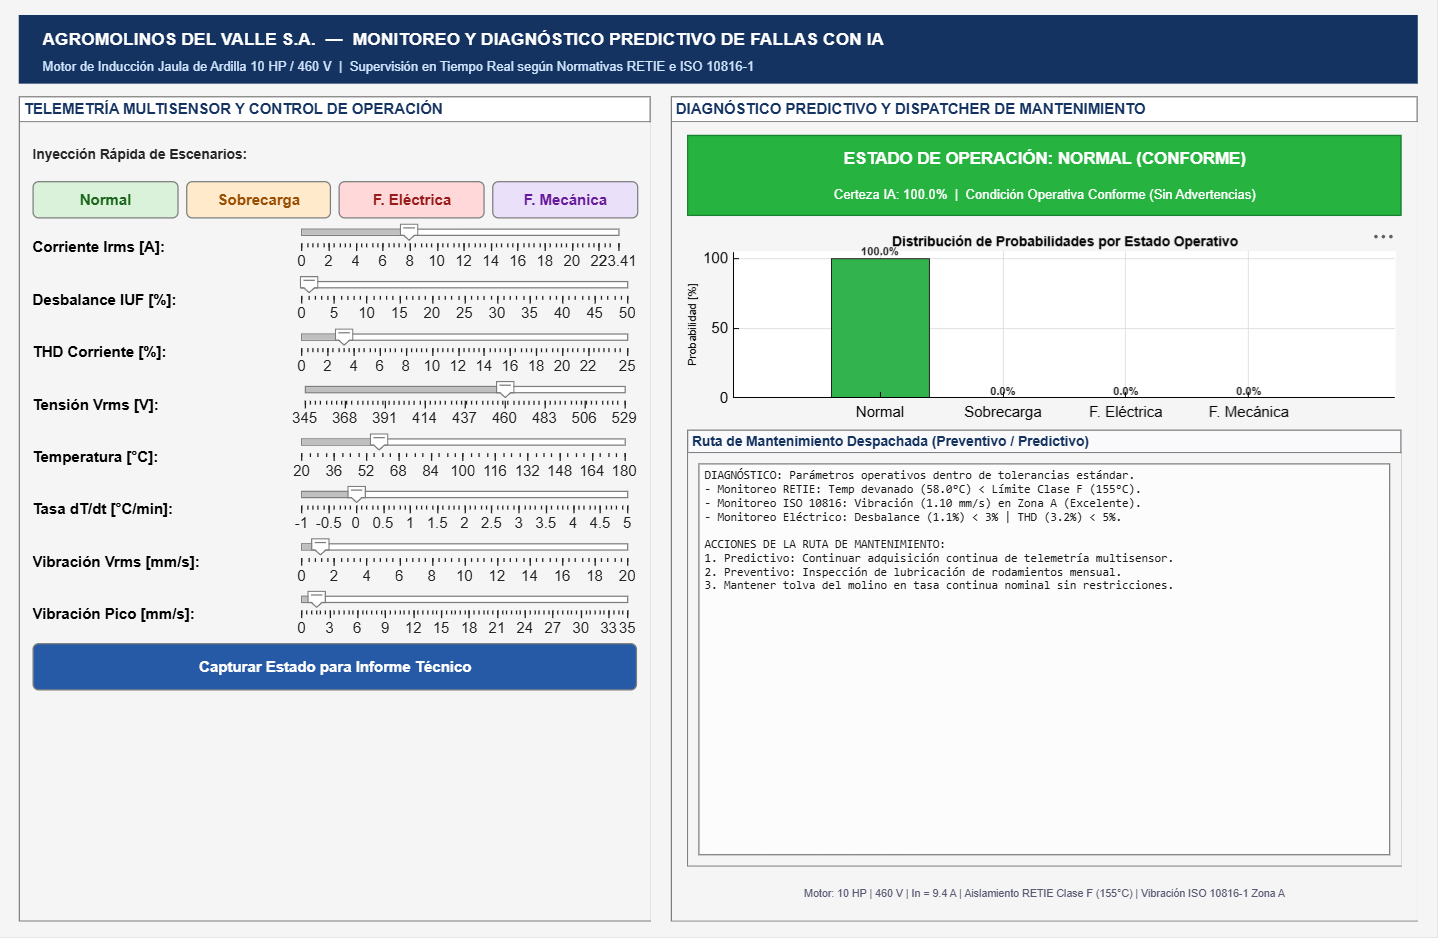
\includegraphics[width=0.98\columnwidth]{interfaz_app_designer.png}
    \caption{Captura del panel de control interactivo desarrollado en MATLAB App Designer en modo de operación normal (conforme), desplegando la telemetría multisensor, la clasificación neuronal y la ruta de mantenimiento preventivo y predictivo.}
    \label{fig:interfaz_app}
\end{figure}

\section{Conclusiones}
Los resultados obtenidos validan la integración del control dinámico, el diagnóstico predictivo mediante Inteligencia Artificial y la gestión normativa del mantenimiento para el motor de 10~HP en AgroMolinos del Valle S.A.:

\begin{enumerate}
    \item \textbf{Robustez y Agilidad del Control Directo de Par (DTC):} La integración del modelo electromecánico en Simulink confirmó la eficacia del control por histéresis y la sintonización analítica del lazo PI de velocidad ($\zeta = 1.0, \omega_n = 20$). Frente al escalón de carga nominal ($T_n = 39.58~\text{N\,m}$) en $t = 1.0$~s y la posterior sobrecarga por atasco ($1.35 T_n = 53.43~\text{N\,m}$) en $t = 1.60$~s, el accionamiento restituyó el balance de par en menos de $15$~ms y compensó la caída transitoria de velocidad ($\Delta\omega = -3.75\%$) en $150$~ms, manteniendo la regulación dentro de la banda del $\pm 2\%$, lo que certifica la capacidad del lazo para soportar los transitorios severos inherentes a la molienda de granos.
    \item \textbf{Eficacia Diagnóstica del Vector de Características e Inteligencia Artificial:} La estructuración del vector $\mathbf{x} \in \mathbb{R}^8$ integrando magnitudes eléctricas ($I_{rms}, IUF, THD_i, V_{rms}$), térmicas ($T_{dev}, dT/dt$) y mecánicas ($v_{rms}, v_{peak}$), complementada con la estandarización $Z$-Score, demostró una capacidad de discriminación completa. Tanto el Perceptrón Multicapa ($8 \to 16 \to 8 \to 4$) entrenado con el optimizador Adam ($\mathcal{L} \to 10^{-4}$) como la SVM OvR con kernel RBF alcanzaron un $100.0\%$ de exactitud, precisión, sensibilidad y F1-score sobre los 240 casos de prueba ciega. La proyección mediante PCA ratificó la formación de agrupamientos disjuntos y convexos con más del $85\%$ de varianza explicada, comprobando que las fallas eléctricas, térmicas y mecánicas poseen firmas físicas desacopladas \cite{soualhi2022, gangsar2020}.
    \item \textbf{Alineación Normativa y Ruta de Mantenimiento Basada en Condición:} Las directrices del RETIE Art.~20 (límite de $155^\circ$C para aislamiento Clase F) y de la norma ISO 10816-1 (límite admisible de $1.8$~mm/s y umbral de alarma crítica en $4.5$~mm/s) se tradujeron en compuertas de decisión automatizadas. La Ruta de Mantenimiento articula un protocolo de dos niveles: contención operativa inmediata en planta (reducción de tolva, parada LOTO o desacople) e intervención electromecánica especializada en taller (ensayos CoreLoss $<2.0$~W/kg, pirólisis en horno BurnOut a $370^\circ$C, rebobinado CNC, barnizado VPI y alineación láser $<0.05$~mm), minimizando paradas imprevistas y resguardando la vida útil del activo.
    \item \textbf{Viabilidad Operativa y Despliegue en MATLAB App Designer:} La interfaz gráfica desarrollada bajo arquitectura de espacio de trabajo estático sincronizada con el archivo maestro \texttt{InductionMachineDTCData.m} ofrece una herramienta de doble propósito: plataforma de simulación para inyección de anomalías y consola de supervisión en tiempo real lista para su implementación en controladores industriales de borde (DSP/PLC). El semáforo de estado, la visualización probabilística y el filtrado por certeza ($P \ge 90\%$) facilitan la toma de decisiones ágil y confiable por parte del personal de planta.
\end{enumerate}

\newpage
\appendices

\section{Archivo Maestro de Parámetros (\texttt{InductionMachineDTCData.m})}
\label{app:dtcdata}
El siguiente código representa la Única Fuente de Verdad Paramétrica del motor y de los lazos DTC:
\begin{lstlisting}[caption={Script maestro de constantes paramétricas (\texttt{InductionMachineDTCData.m})}, label={lst:dtcdata}]
Pn = 7460; Vn = 460; fn = 60; p = 2;
Rs = 0.0139; Lls = 0.0672; Rr = 0.0112; Llr = 0.0672; Lm = 2.717;
Lr = Llr + Lm; Ls = Lls + Lm;
H = 0.2734; F = 0.0106;

Vbase = Vn / sqrt(3) * sqrt(2);
Ibase = Pn / (1.5 * Vbase);
Zbase = Vbase / Ibase;
wbase = 2 * pi * fn;
Tbase = Pn / (wbase / p);
psin  = Vbase / wbase;

Rss = Rs * Zbase; Xls = Lls * Zbase;
Rrr = Rr * Zbase; Xlr = Llr * Zbase; Xm = Lm * Zbase;

Ts = 5e-6; fsw = 2e3; Tsc = Ts;
zeta = 1.0; wn = 20;
Kp_wr = 2 * zeta * wn * (2 * H) - F;
Ki_wr = (wn^2) * (2 * H);
FluxHystBand = 0.015;
THystBand = 3;
\end{lstlisting}

\newpage
\section{Sintonización Analítica del Lazo PI (\texttt{tune\_pi.m})}
\label{app:tunepi}
Rutina que mapea el modelo mecánico rotacional al dominio de Laplace para determinar las ganancias del regulador de velocidad:
\begin{lstlisting}[caption={Sintonización del regulador PI de velocidad (\texttt{tune\_pi.m})}, label={lst:tunepi}]
InductionMachineDTCData;
wbase_mech = 2 * pi * fn / p;
Tbase = Pn / wbase_mech;
J = (2 * H * Tbase) / wbase_mech;
F_si = F * (Tbase / wbase_mech);

K_planta = Tbase / J;
a_planta = F_si / J;

tiempos_deseados = [0.05, 0.1, 0.2, 0.5];
zeta = 1.0;
for ts = tiempos_deseados
    wn = 4 / (zeta * ts);
    Kp_calc = (2 * zeta * wn - a_planta) / K_planta;
    Ki_calc = (wn^2) / K_planta;
    fprintf('ts = %.2f s -> Kp = %.4f, Ki = %.4f\n', ts, Kp_calc, Ki_calc);
end
\end{lstlisting}

\newpage
\section{Generador Dinámico del Dataset de Fallas (\texttt{generate\_dataset.m})}
\label{app:gen}
Rutina de emulación física de los cuatro estados de operación sincronizada dinámicamente con \texttt{InductionMachineDTCData.m}:
\begin{lstlisting}[caption={Generador de dataset de fallas multivariable (\texttt{generate\_dataset.m})}, label={lst:gen}]
clear; rng(42);
simPath = fullfile(fileparts(mfilename('fullpath')), '..', 'simulaciones');
addpath(simPath); InductionMachineDTCData;

In_rms = Ibase / sqrt(2); Tn = Tbase;
nSamples = 300; N = nSamples * 4;
X = zeros(N, 8); Y = zeros(N, 1);

for i = 1:nSamples
    lf = 0.20 + 0.80 * rand();
    X(i,:) = [(0.35*In_rms + 0.65*In_rms*lf)+0.25*randn(), 0.5+1.2*rand()+0.15*abs(randn()), ...
              2.0+2.0*rand()+0.25*randn(), Vn+3.5*randn(), 40+32*lf+2.0*randn(), ...
              0.05*randn(), 0.70+0.75*lf+0.12*randn(), (0.70+0.75*lf)*(1.35+0.15*rand())];
    Y(i) = 1;
end
for i = 1:nSamples
    idx = nSamples + i; ov = 1.15 + 0.45 * rand();
    X(idx,:) = [In_rms*ov+0.4*randn(), 1.0+1.5*rand()+0.2*randn(), 3.5+1.8*rand()+0.35*randn(), ...
                Vn-3+4.5*randn(), 98+52*(ov-1.15)/0.45+3*randn(), 1.2+2.3*rand()+0.25*abs(randn()), ...
                1.4+0.8*rand()+0.15*randn(), (1.4+0.8*rand())*(1.4+0.2*rand())];
    Y(idx) = 2;
end
for i = 1:nSamples
    idx = 2*nSamples + i; sev = 0.20 + 0.80 * rand();
    X(idx,:) = [In_rms*(0.85+0.55*sev)+0.5*randn(), 8.0+34.0*sev+1.2*randn(), ...
                6.0+11.0*sev+0.8*randn(), Vn-15*sev+5.0*randn(), 65+35*sev+2.5*randn(), ...
                0.4+1.0*sev+0.15*randn(), 2.0+2.0*sev+0.25*randn(), (2.0+2.0*sev)*(1.6+0.3*rand())];
    Y(idx) = 3;
end
for i = 1:nSamples
    idx = 3*nSamples + i; ms = 0.20 + 0.80 * rand();
    X(idx,:) = [In_rms*(0.90+0.30*ms)+0.35*randn(), 1.5+2.5*ms+0.25*randn(), ...
                3.0+3.5*ms+0.35*randn(), Vn+3.0*randn(), 55+26*ms+2.0*randn(), ...
                0.2+0.45*ms+0.1*randn(), 4.2+8.5*ms+0.35*randn(), (4.2+8.5*ms)*(2.1+1.1*rand())];
    Y(idx) = 4;
end
X(:, [1,2,3,4,5,7,8]) = max(X(:, [1,2,3,4,5,7,8]), 0.01);
shuff = randperm(N); X = X(shuff, :); Y = Y(shuff);
featureNames = {'Irms_A','IUF_pct','THD_pct','Vrms_V','Temp_C','dTemp_dt','Vrms_vib_mms','Vpeak_vib_mms'};
classNames = {'Normal','Sobrecalentamiento','Falla_Electrica','Falla_Mecanica'};
save('motor_fault_dataset.mat', 'X', 'Y', 'featureNames', 'classNames', 'Pn', 'Vn', 'fn', 'In_rms', 'Tn');
\end{lstlisting}

\newpage
\section{Entrenamiento de Red Neuronal y SVM (\texttt{train\_classifiers.m})}
\label{app:train}
Implementación nativa de la red neuronal MLP (optimizador Adam) y SVM (One-vs-Rest Gaussiana):
\begin{lstlisting}[caption={Entrenamiento de modelos supervisados (\texttt{train\_classifiers.m})}, label={lst:train}]
clear; rng(42); load('motor_fault_dataset.mat');
[N, numFeatures] = size(X); numClasses = length(classNames);
idxTrain = []; idxTest = [];
for c = 1:numClasses
    cIdx = find(Y == c); nTrain = round(0.80 * length(cIdx));
    p_perm = randperm(length(cIdx));
    idxTrain = [idxTrain; cIdx(p_perm(1:nTrain))];
    idxTest  = [idxTest;  cIdx(p_perm(nTrain+1:end))];
end
mu = mean(X(idxTrain, :), 1); sigma = std(X(idxTrain, :), 0, 1);
sigma(sigma == 0) = 1;
X_train_norm = (X(idxTrain, :) - mu) ./ sigma;
X_test_norm  = (X(idxTest, :)  - mu) ./ sigma;
Y_train_oh = eye(numClasses); Y_train_oh = Y_train_oh(Y(idxTrain), :);
Y_test_oh  = eye(numClasses); Y_test_oh  = Y_test_oh(Y(idxTest), :);

W1 = randn(8, 16)*sqrt(2/8);  b1 = zeros(1, 16);
W2 = randn(16, 8)*sqrt(2/16); b2 = zeros(1, 8);
W3 = randn(8, 4)*sqrt(2/8);   b3 = zeros(1, 4);
mW1 = zeros(size(W1)); vW1 = zeros(size(W1)); mb1 = zeros(size(b1)); vb1 = zeros(size(b1));
mW2 = zeros(size(W2)); vW2 = zeros(size(W2)); mb2 = zeros(size(b2)); vb2 = zeros(size(b2));
mW3 = zeros(size(W3)); vW3 = zeros(size(W3)); mb3 = zeros(size(b3)); vb3 = zeros(size(b3));

epochs = 350; batchSize = 32; lr = 0.008; lambda_reg = 1e-4;
m_tr = size(X_train_norm, 1);
for ep = 1:epochs
    sh = randperm(m_tr); X_sh = X_train_norm(sh, :); Y_sh = Y_train_oh(sh, :);
    for b = 1:ceil(m_tr/batchSize)
        idx_b = (b-1)*batchSize + 1 : min(b*batchSize, m_tr);
        xb = X_sh(idx_b, :); yb = Y_sh(idx_b, :); mb = size(xb, 1);
        z1 = xb*W1 + b1; a1 = max(0, z1);
        z2 = a1*W2 + b2; a2 = max(0, z2);
        z3 = a2*W3 + b3; ez3 = exp(z3 - max(z3,[],2)); a3 = ez3 ./ sum(ez3, 2);
        dz3 = (a3 - yb)/mb; dW3 = a2'*dz3 + lambda_reg*W3; db3 = sum(dz3, 1);
        dz2 = (dz3*W3') .* (z2 > 0); dW2 = a1'*dz2 + lambda_reg*W2; db2 = sum(dz2, 1);
        dz1 = (dz2*W2') .* (z1 > 0); dW1 = xb'*dz1 + lambda_reg*W1; db1 = sum(dz1, 1);
        t_step = (ep-1)*ceil(m_tr/batchSize) + b;
        mW3 = 0.9*mW3 + 0.1*dW3; vW3 = 0.999*vW3 + 0.001*(dW3.^2);
        W3 = W3 - lr*(mW3/(1-0.9^t_step)) ./ (sqrt(vW3/(1-0.999^t_step)) + 1e-8);
        b3 = b3 - lr*db3;
        mW2 = 0.9*mW2 + 0.1*dW2; vW2 = 0.999*vW2 + 0.001*(dW2.^2);
        W2 = W2 - lr*(mW2/(1-0.9^t_step)) ./ (sqrt(vW2/(1-0.999^t_step)) + 1e-8);
        b2 = b2 - lr*db2;
        mW1 = 0.9*mW1 + 0.1*dW1; vW1 = 0.999*vW1 + 0.001*(dW1.^2);
        W1 = W1 - lr*(mW1/(1-0.9^t_step)) ./ (sqrt(vW1/(1-0.999^t_step)) + 1e-8);
        b1 = b1 - lr*db1;
    end
end
z1 = max(0, X_test_norm*W1 + b1); z2 = max(0, z1*W2 + b2);
ez3 = exp(z2*W3 + b3 - max(z2*W3 + b3,[],2)); probs = ez3 ./ sum(ez3, 2);
[~, pred_ann] = max(probs, [], 2);
ann_accuracy = mean(pred_ann == Y(idxTest)) * 100;
model_ann = struct('W1',W1,'b1',b1,'W2',W2,'b2',b2,'W3',W3,'b3',b3,'mu',mu,'sigma',sigma,...
                   'featureNames',{featureNames},'classNames',{classNames},'accuracy',ann_accuracy);
save('modelo_ia_entrenado.mat', 'model_ann', 'ann_accuracy');
\end{lstlisting}

\section{Panel Interactivo de App Designer (\texttt{MotorFaultDiagnosticGUI.m})}
\label{app:gui}
Interfaz gráfica de usuario para monitoreo multisensor y despacho de la ruta de mantenimiento:
\begin{lstlisting}[caption={Panel de control y despacho predictivo (\texttt{MotorFaultDiagnosticGUI.m})}, label={lst:gui}]
function app = MotorFaultDiagnosticGUI(options)
    arguments
        options.AutoSaveSnapshot (1,1) logical = false
        options.SnapshotPath (1,1) string = fullfile(fileparts(mfilename('fullpath')), '..', 'imagenes', 'interfaz_app_designer.png')
    end
    currentDir = fileparts(mfilename('fullpath'));
    simPath = fullfile(currentDir, '..', 'simulaciones');
    motorParams = loadMotorConstants(fullfile(simPath, 'InductionMachineDTCData.m'));
    Pn = motorParams.Pn; Vn = motorParams.Vn; Ibase = motorParams.Ibase;
    In_rms = Ibase / sqrt(2);
    dataLoaded = load(fullfile(currentDir, 'modelo_ia_entrenado.mat'));
    model = dataLoaded.model_ann;

    fig = uifigure('Name', sprintf('AgroMolinos del Valle S.A. - Monitoreo Predictivo Motor %0.0f HP', Pn/746), ...
                   'Position', [80, 60, 1150, 720], 'Color', [0.95, 0.96, 0.98]);
    mainGrid = uigridlayout(fig, [1, 2]); mainGrid.ColumnWidth = {'1.1x', '1.3x'};
    
    leftPanel = uipanel(mainGrid, 'Title', 'TELEMETRIA Y CONTROL OPERATIVO', 'FontWeight', 'bold');
    leftGrid = uigridlayout(leftPanel, [12, 2]); leftGrid.RowHeight = {35, 30, 42, 42, 42, 42, 42, 42, 42, 42, 40, '1x'};
    btnGrid = uigridlayout(leftGrid, [1, 4]); btnGrid.Layout.Row = 2; btnGrid.Layout.Column = [1, 2];
    uibutton(btnGrid, 'Text', 'Normal', 'ButtonPushedFcn', @(~,~) setScenario('Normal'));
    uibutton(btnGrid, 'Text', 'Sobrecarga', 'ButtonPushedFcn', @(~,~) setScenario('Sobrecalentamiento'));
    uibutton(btnGrid, 'Text', 'F. Electrica', 'ButtonPushedFcn', @(~,~) setScenario('Falla_Electrica'));
    uibutton(btnGrid, 'Text', 'F. Mecanica', 'ButtonPushedFcn', @(~,~) setScenario('Falla_Mecanica'));

    uilabel(leftGrid, 'Text', 'Corriente Irms [A]:');
    sldIrms = uislider(leftGrid, 'Limits', [0, In_rms*2.5], 'Value', In_rms*0.8, 'ValueChangedFcn', @(~,~) updateDiagnosis());
    uilabel(leftGrid, 'Text', 'Desbalance IUF [%]:');
    sldIUF = uislider(leftGrid, 'Limits', [0, 50], 'Value', 1.2, 'ValueChangedFcn', @(~,~) updateDiagnosis());
    uilabel(leftGrid, 'Text', 'THD Corriente [%]:');
    sldTHD = uislider(leftGrid, 'Limits', [0, 25], 'Value', 3.0, 'ValueChangedFcn', @(~,~) updateDiagnosis());
    uilabel(leftGrid, 'Text', 'Tension Vrms [V]:');
    sldVrms = uislider(leftGrid, 'Limits', [Vn*0.75, Vn*1.15], 'Value', Vn, 'ValueChangedFcn', @(~,~) updateDiagnosis());
    uilabel(leftGrid, 'Text', 'Temperatura [C]:');
    sldTemp = uislider(leftGrid, 'Limits', [20, 180], 'Value', 58, 'ValueChangedFcn', @(~,~) updateDiagnosis());
    uilabel(leftGrid, 'Text', 'Tasa dT/dt [C/min]:');
    sldGrad = uislider(leftGrid, 'Limits', [-1.0, 5.0], 'Value', 0.0, 'ValueChangedFcn', @(~,~) updateDiagnosis());
    uilabel(leftGrid, 'Text', 'Vibracion Vrms [mm/s]:');
    sldVibRMS = uislider(leftGrid, 'Limits', [0, 20], 'Value', 1.1, 'ValueChangedFcn', @(~,~) updateDiagnosis());
    uilabel(leftGrid, 'Text', 'Vibracion Pico [mm/s]:');
    sldVibPeak = uislider(leftGrid, 'Limits', [0, 35], 'Value', 1.6, 'ValueChangedFcn', @(~,~) updateDiagnosis());

    pnlHeader = uipanel(mainGrid, 'BackgroundColor', [0.08, 0.20, 0.38], 'BorderType', 'none');
    uilabel(pnlHeader, 'Text', 'AGROMOLINOS DEL VALLE S.A. -- MONITOREO Y DIAGNOSTICO CON IA', ...
            'FontSize', 14, 'FontWeight', 'bold', 'FontColor', 'w', 'Position', [20, 26, 1080, 22]);
    uilabel(pnlHeader, 'Text', 'Motor 10 HP / 460 V | Supervision RETIE e ISO 10816-1', ...
            'FontSize', 10, 'FontColor', [0.82, 0.90, 1.0], 'Position', [20, 6, 1080, 18]);

    bodyGrid = uigridlayout(mainGrid, [1, 2]); bodyGrid.ColumnWidth = {'1.1x', '1.3x'};
    leftPanel = uipanel(bodyGrid, 'Title', 'TELEMETRIA MULTISENSOR', 'FontWeight', 'bold');
    rightPanel = uipanel(bodyGrid, 'Title', 'DIAGNOSTICO IA Y RUTA DE MANTENIMIENTO', 'FontWeight', 'bold');
    rightGrid = uigridlayout(rightPanel, [4, 1]); rightGrid.RowHeight = {65, 155, '1x', 25};
    pnlBanner = uipanel(rightGrid, 'BackgroundColor', [0.15, 0.70, 0.25], 'AutoResizeChildren', 'off');
    lblStatusTitle = uilabel(pnlBanner, 'Text', 'ESTADO: NORMAL (CONFORME)', 'FontWeight', 'bold', ...
                             'FontColor', 'w', 'FontSize', 13.5, 'HorizontalAlignment', 'center', 'Position', [10, 34, 570, 24]);
    lblConfidence = uilabel(pnlBanner, 'Text', 'Certeza: 100%', 'FontColor', 'w', 'FontSize', 10.5, ...
                            'HorizontalAlignment', 'center', 'Position', [10, 8, 570, 20]);
    axProbs = uiaxes(rightGrid); axProbs.YLim = [0, 105];
    txtMaint = uitextarea(rightGrid, 'Editable', 'off', 'FontName', 'Consolas');

    function updateDiagnosis()
        x_raw = [sldIrms.Value, sldIUF.Value, sldTHD.Value, sldVrms.Value, sldTemp.Value, sldGrad.Value, sldVibRMS.Value, sldVibPeak.Value];
        x_norm = (x_raw - model.mu) ./ model.sigma;
        z1 = max(0, x_norm * model.W1 + model.b1);
        z2 = max(0, z1 * model.W2 + model.b2);
        ez3 = exp(z2 * model.W3 + model.b3 - max(z2 * model.W3 + model.b3));
        probs = (ez3 ./ sum(ez3)) * 100; [maxProb, predIdx] = max(probs);
        b = bar(axProbs, 1:4, probs, 'FaceColor', 'flat');
        b.CData = [0.2 0.7 0.3; 0.95 0.55 0.1; 0.85 0.2 0.2; 0.6 0.2 0.8];
        axProbs.XTickLabel = {'Normal', 'Sobrecarga', 'F. Electrica', 'F. Mecanica'};
        switch model.classNames{predIdx}
            case 'Normal'
                pnlBanner.BackgroundColor = [0.15, 0.70, 0.25];
                lblStatusTitle.Text = 'ESTADO: NORMAL (CONFORME)';
                txtMaint.Value = 'Operacion nominal en molino. Tareas preventivas mensuales.';
            case 'Sobrecalentamiento'
                pnlBanner.BackgroundColor = [0.92, 0.50, 0.08];
                lblStatusTitle.Text = 'ALERTA: SOBRECALENTAMIENTO TERMICO';
                txtMaint.Value = 'Reducir tolva al 60%. Desobstruir ventilacion. Limite RETIE Clase F (155 C).';
            case 'Falla_Electrica'
                pnlBanner.BackgroundColor = [0.85, 0.15, 0.15];
                lblStatusTitle.Text = 'CRITICO: ASIMETRIA / FALLA ELECTRICA';
                txtMaint.Value = 'Parada LOTO. Envio a Taller: CoreLoss Test, Horno BurnOut 370 C, Rebobinado CNC, VPI.';
            case 'Falla_Mecanica'
                pnlBanner.BackgroundColor = [0.55, 0.15, 0.75];
                lblStatusTitle.Text = 'URGENTE: FALLA MECANICA / ROZAMIENTO';
                txtMaint.Value = 'Desacople. Reemplazo rodamientos C3, alineacion laser (< 0.05 mm), balanceo dinamico.';
        end
        lblConfidence.Text = sprintf('Certeza IA: %.1f%%', maxProb);
    end
    setScenario('Normal');
    if nargout > 0, app = fig; end
end
function params = loadMotorConstants(scriptPath)
    run(scriptPath); params = struct('Pn',Pn,'Vn',Vn,'fn',fn,'p',p,'Tbase',Tbase,'Ibase',Ibase,'Rs',Rs);
end
\end{lstlisting}

\section{Script de Lanzamiento Rápido (\texttt{abrir\_panel.m})}
\label{app:abrir}
Script simplificado para abrir el panel interactivo desde la consola de MATLAB:
\begin{lstlisting}[caption={Script de inicialización y apertura del panel (\texttt{abrir\_panel.m})}, label={lst:abrir}]
clc;
rootDir = fileparts(mfilename('fullpath'));
simDir  = fullfile(rootDir, 'Informe', 'simulaciones');
iaDir   = fullfile(rootDir, 'Informe', 'IA');
addpath(simDir); addpath(iaDir);

if ~isfile(fullfile(iaDir, 'modelo_ia_entrenado.mat'))
    run(fullfile(iaDir, 'train_classifiers.m'));
end
app = MotorFaultDiagnosticGUI();
\end{lstlisting}

\bibliographystyle{IEEEtran}
\bibliography{IEEEabrv,referencias}

\end{document}

